% ==============================================
\section*{Chapter 2}
% ==============================================

\iffalse
% ---------------------------------------
\Soln{Non-Perturbative Effects}{lqcd-nonpert}
% ---------------------------------------

% ---------------------------------------
\Soln{Leading Order Results for \texorpdfstring{\(e^+\,e^-\)}{electron-positron} to hadrons}{eetohadrons_lo}
% ---------------------------------------

First, let us recall the diagram for the process in question,
%
\begin{align}
    \tikzexdiagram{ee_to_qq}[0][1.3]
\end{align}
and recall the Feynman rules of QCD:
\sam{include}

Assuming all partons are massless and working in Feynman gauge,
\begin{subequations}
\begin{align}
    i \mathcal{M}_2^{(0)}
    &=
    \le(
    -i e_q
    \gamma^\mu
    \ri)
    \frac{i\eta_{\mu\nu}}{\le(p_1 + p_2\ri)^2}
    \le(
    -i e_q
    \gamma^\nu
    \ri)
    \\
    &=
\end{align}
\end{subequations}
\sam{missing spinor factors}
\sam{missing color factors}






% ---------------------------------------
\Soln{Next-to-Leading Order Results for \texorpdfstring{\(e^+\,e^-\)}{electron-positron} to hadrons}{eetohadrons_nlo}
% ---------------------------------------

% https://zzxianyu.com/wp-content/uploads/2017/01/peskin_problems.pdf#page=75

\begin{align}
    \tikzexdiagram{ee_to_qqg}[0][1.0]
\end{align}


\begin{align}
    \,.
\end{align}



\begin{align}
    \tikzexdiagram{ee_to_qq_loop}[0][1.5]
\end{align}



\begin{align}
    i \mathcal{M}_2^{(2)}
    =
    -i e
    \le(-i e_q\ri)
    \le(-i g_s\ri)^2
    \,\,
    \le(
    \gamma^\mu
    \ri)
    \,\,
    \frac{i \eta_{\mu\nu}}{\le(p_1 + p_2\ri)^2}
    \,\,
    \le(
        (T_F^a)\indices{^i_k}
        \,\,
        \gamma^\rho
        \,\,
        \frac{i \le(\slashed{k_1} + \slashed{\ell}\ri)}
            {\le(k_1 + \ell\ri)^2}
        \,\,
        \gamma^\nu
        \,\,
        \frac{i \le(\slashed{k_2} - \slashed{\ell}\ri)}
            {\le(k_2 - \ell\ri)^2}
        \,\,
        \gamma^\sigma
        \,\,
        (T_F^b)\indices{^k_j}
    \ri)
    \,\,
    \frac{i \delta_{ab} \eta_{\rho\sigma}}{\ell^2}
    \,.
\end{align}


% ---------------------------------------
\Soln{Kinematics for \texorpdfstring{\(e^+\,e^-\)}{electron-positron} to hadrons at NLO}{eetohadrons_kinematics}
% ---------------------------------------

Notice that
\begin{align}
    (p_i + p_j)^2 = 2 E_i E_j (1 - \cos\theta_{ij}) = \frac{1}{2}Q^2 x_i x_j (1 - \cos\theta_{ij})
    \,,
\end{align}
which by momentum conservation is
\begin{align}
    (q - p_{\overline{ij}})^2 = Q^2 - 2 Q E_{\overline{ij}} = Q^2(1 - x_{\overline{ij}}) = Q^2(x_i + x_j - 1).
\end{align}
where \(p_{\overline{ij}}\) is the momentum of the final state which is not \(i\) or \(j\)
%
--
%
for example, if \(i=q\) and \(j = g\), then \(\overline{ij} = \bar{q}\), while if \(i=q\) and \(j = \bar{q}\), then \(\overline{ij} = g\).

Equating these formulae quickly yields
\begin{align}
    \cos\theta_{ij} &= \frac{1}{x_i x_j} - \frac{2}{x_i} - \frac{2}{x_j} + 1
    ,
    \\
    \frac{m^2_{ij}}{Q^2} &= x_i + x_j - 1
    .
\end{align}

The Lorentz-invariant form of these equations can be quickly written by noting that \(x_i = 2 E_i/\sqrt{s} = \frac{2 p_i\cdot q}{q^2}\), since, in the center of mass frame, the photon has momentum \(q \reppedby \sqrt{s}(1,0,0,0)\).



% ---------------------------------------
\Soln{Factorization of Collinear Phase Space}{phase-space-factorization}
% ---------------------------------------

% ---------------------------------------
\Soln{A Physical Approach to Plus-Functions}{physics-plus}
% ---------------------------------------

% ---------------------------------------
\Soln{Splitting Functions in Dimensional Regularisation}{dimreg-splitting}
% ---------------------------------------
\fi

% ---------------------------------------
\Soln{Massless Splitting Functions in \texorpdfstring{\(\phi^3\)}{phi-cubed} Theory}{phi-cubed-splitting}
% ---------------------------------------

\newcommand{\phicubedsix}{\ensuremath{\le(\phi^3\ri)_{d=6}}}


Consider the \textbf{\(\phi^3\) theory in \(d=5+1\) dimensions} with coupling constant \(g\):
\begin{align}
    \mathcal{L}
    =
    -\frac{1}{2}\le(\partial_\mu \phi \partial^\mu \phi\ri)
    -
    \frac{1}{2}m^2 \phi^2
    -
    \frac{g}{3!}\phi^3
    .
\end{align}
Henceforth, we will refer to this model affectionately as \phicubedsix.

\phicubedsix{} echoes some of the features of branchings in gauge theories which produce jets:
\begin{itemize}
    \item
    it has three-point vertices which allow ``branchings'', as we will see, which are reminiscent of the splittings which produce jets in the standard model;

    \item
    crucially, it has \vocab{collinear divergences}:
    %
    scattering amplitudes have divergent behavior in the limit where any pair of external particles have nearly collinear momenta.
\end{itemize}


Let's start by looking how matter can branch into other matter in \phicubedsix{}.
%
Roughly, we will see that the structure of the Feynman rules will allow us to relate higher-point amplitudes to lower point amplitudes, and that cross sections for physical scattering will be dominated by regions of phase space where two particles are nearly collinear.


Let's examine the amplitude
\begin{align}
    \begin{tikzpicture}[baseline={(0,-0.1)}]
        \begin{feynman}
            \node[blob] (mid) {};
            \vertex (a) [above left=of mid] {\(p_1\)};
            \vertex (b) [below left=of mid] {\(p_m\)};
            \vertex (c) [above right=of mid] {\(k_n\)};
            \vertex (d) [below right=of mid] {\(k_1\)};
            \node[below=1cm of a] (L) {\(\vdots\)};
            \node[below=1cm of c] (L) {\(\vdots\)};
            \diagram* {
                (a) -- (mid) -- (b),
                (d) -- (mid) -- (c),
            };
        \end{feynman}
    \end{tikzpicture}
    \,
    =
    \,\,\,
    \widetilde{\mc{M}}_{m\to n}(p_1,\cdots,p_m;\,k_1,\cdots,k_n)
    \,\,
    .
\end{align}
We will deal only with connected amplitudes in what follows.

Note that the only way to produce a \(\widetilde{\mc{M}}_{m \to n}\), at least perturbatively, is to use the cubic vertex of \phicubedsix{} to produce new outgoing lines from lower-order amplitudes:
\begin{align}
    \widetilde{\mc{M}}_{m\to n}(p_1,\cdots,p_m;\,k_1,\cdots,k_n)
    \,\,
    =
    \begin{tikzpicture}[baseline={(0,-0.1)}]
        \begin{feynman}
            \node[blob] (mid) {};
            \vertex (a) [above left=of mid] {\(p_1\)};
            \vertex (ap) [below right=.5cm and .5cm of a];
            \vertex (b) [below left=of mid] {\(p_m\)};
            \vertex (c) [above right=of mid] {\(k_n\)};
            \vertex (cp) [below=.7cm of c] {\(k_{n-1}\)};
            \vertex (d) [below right=of mid] {\(k_1\)};
            \node[below=1cm of a] (L) {\(\vdots\)};
            \node[below=1.2cm of c] (L) {\(\vdots\)};
            \diagram* {
                (a) -- (mid) -- (b),
                (d) -- (mid),
                (ap) -- (c),
                (mid) -- (cp),
            };
        \end{feynman}
    \end{tikzpicture}
    \quad
    +
    \quad
    \begin{tikzpicture}[baseline={(0,-0.1)}]
        \begin{feynman}
            \node[blob] (mid) {};
            \vertex (a) [above left=of mid] {\(p_1\)};
            \vertex (b) [below left=of mid] {\(p_m\)};
            \vertex (cpp) [above right=.4cm and .4cm of mid];
            \vertex (c) [above right=.3cm and .6cm of cpp] {\(k_n\)};
            \vertex (cp) [right=.6cm of cpp] {\(k_{n-1}\)};
            \vertex (d) [below right=of mid] {\(k_1\)};
            \node[below=1cm of a] (L) {\(\vdots\)};
            \node[below left=1.2cm and .3cm of c] (L) {\(\vdots\)};
            \diagram* {
                (a) -- (mid) -- (b),
                (d) -- (mid),
                % (cp) -- (cpp) -- (c)
                (cp) -- (cpp) -- (c),
                (mid) -- (cpp),
            };
        \end{feynman}
    \end{tikzpicture}
    \quad
    +
    \quad
    \cdots
    ,
    \label{eq:eikonal_diagram}
\end{align}
where the ellipses include the diagrams where \(k_n\) branches off of any of the external lines of the lower point amplitude.

\Eq{eikonal_diagram} indicates that the diagrams with \(n+m\) external lines can be produced by starting with diagrams with \(n+m-1\) external lines and including an additional propagator factor.
%
When attaching a new outgoing line to any of the ingoing particles, the propagator involves the difference of two momenta;
%
for example, the first diagram of \Eq{eikonal_diagram} is
\begin{align}
    \begin{tikzpicture}[baseline={(0,-0.1)}]
        \begin{feynman}
            \node[blob] (mid) {};
            \vertex (a) [above left=of mid] {\(p_1\)};
            \vertex (ap) [below right=.5cm and .5cm of a];
            \vertex (b) [below left=of mid] {\(p_m\)};
            \vertex (c) [above right=of mid] {\(k_n\)};
            \vertex (cp) [below=.7cm of c] {\(k_{n-1}\)};
            \vertex (d) [below right=of mid] {\(k_1\)};
            \node[below=1cm of a] (L) {\(\vdots\)};
            \node[below=1.2cm of c] (L) {\(\vdots\)};
            \diagram* {
                (a) -- (mid) -- (b),
                (d) -- (mid),
                (ap) -- (c),
                (mid) -- (cp),
            };
        \end{feynman}
    \end{tikzpicture}
    \quad
    =
    \quad
    \frac{g}{(p_1 - k_n)^2 + m^2}
    \,\,\,\,
    \widetilde{\mc{M}}_{m \to n-1}(p_1 - k_n, p_2,\cdots, p_m;\,k_1,\cdots,k_{n-1})
    .
\end{align}
The additional factor due to the propagator is called an \vocab{eikonal factor}.

When instead attaching our new outgoing external line to the out-going particles, we instead have the sum of two momenta in the propagator
\begin{align}
    \begin{tikzpicture}[baseline={(0,-0.1)}]
        \begin{feynman}
            \node[blob] (mid) {};
            \vertex (a) [above left=of mid] {\(p_1\)};
            \vertex (b) [below left=of mid] {\(p_m\)};
            \vertex (cpp) [above right=.4cm and .4cm of mid];
            \vertex (c) [above right=.3cm and .6cm of cpp] {\(k_n\)};
            \vertex (cp) [right=.6cm of cpp] {\(k_{n-1}\)};
            \vertex (d) [below right=of mid] {\(k_1\)};
            \node[below=1cm of a] (L) {\(\vdots\)};
            \node[below left=1.2cm and .3cm of c] (L) {\(\vdots\)};
            \diagram* {
                (a) -- (mid) -- (b),
                (d) -- (mid),
                % (cp) -- (cpp) -- (c)
                (cp) -- (cpp) -- (c),
                (mid) -- (cpp),
            };
        \end{feynman}
    \end{tikzpicture}
    \quad
    =
    \quad
    \frac{g}{(k_{n-1} + k_n)^2 + m^2}
    \,\,\,\,
    \widetilde{\mc{M}}_{m \to n-1}(p_1, p_2,\cdots, p_m;\,k_1,\cdots,k_{n-1}+k_n)
    .
\end{align}

\begin{exercise*}
    Show that
    \begin{align}
        \begin{tikzpicture}[baseline={(0,-0.1)}]
            \begin{feynman}
                \node[blob] (mid) {};
                \vertex (a) [above left=of mid] {\(p_1\)};
                \vertex (b) [below left=of mid] {\(p_m\)};
                \vertex (cpp) [above right=.4cm and .4cm of mid];
                \vertex (c) [above right=.3cm and .6cm of cpp] {\(k_n\)};
                \vertex (cp) [right=.6cm of cpp] {\(k_{n-1}\)};
                \vertex (d) [below right=of mid] {\(k_1\)};
                \node[below=1cm of a] (L) {\(\vdots\)};
                \node[below left=1.2cm and .3cm of c] (L) {\(\vdots\)};
                \diagram* {
                    (a) -- (mid) -- (b),
                    (d) -- (mid),
                    % (cp) -- (cpp) -- (c)
                    (cp) -- (cpp) -- (c),
                    (mid) -- (cpp),
                };
            \end{feynman}
        \end{tikzpicture}
        \!\!
        =
        \frac{g}{2 E_n E_{n-1}(1 - \cos\theta)}
        \widetilde{\mc{M}}_{m \to n-1}(p_1, p_2,\cdots, p_m;\,k_1,\cdots,k_{n-1}+k_n)
    \end{align}
    in the massless limit.
    %
    What is \(\theta\)?

    \indent
    In the massless theory, argue that in the region of phase space where two of the outgoing particles are nearly collinear, the amplitude therefore divides into a singular piece and a lower-point amplitude.
\end{exercise*}

~\\

\begin{exercise*}
    What are the mass dimensions of \(\widetilde{\mc{M}}_{m\to n}\)?
    %
    Ensure that these mass dimensions make sense when combined with the formulae above.
\end{exercise*}


To produce physical predictions about scattering in our theory, it is very useful to use the differential cross section.
%
\textbf{For this purpose, we will restrict ourselves to \(2 \to n\) scattering.}
%
It is useful to remember that, roughly, the differential cross section for measuring a certain outcome is proportional to the probability density of that outcome in a scattering experiment.

Remember that the differential cross section for \(2 \to n\) scattering is given by
\begin{align}
    \dd \sigma_n
    =
    \frac{1}{u_\alpha 2 E_{p_1} 2 E_{p_2}} \le(2\pi\ri)^d
    \delta^{(d)}\le(k_1 + \cdots + k_n - p_1 - p_2\ri)
    \le|
        \widetilde{\mc{M}}_{2 \to n}
    \ri|
    \,
    \dd\widetilde{\Phi}_n
    ,
\end{align}
where \(u_\alpha\) is a ``relative velocity'' which depends only on the initial state, and
\begin{align}
    \dd\widetilde\Phi_n
    =
    \prod_{i=1}^n
    \frac{\dd^{d-1}k_i}{2 E_i \le(2\pi\ri)^{d-1}}
    .
\end{align}

Previously, we saw that amplitudes could be decomposed into lower-point amplitudes and an eikonal factor.
%
A similar decomposition can be made for the phase space measure.

This was done in \Sec{eikonal-limit}, so let us do it in a slightly different way,
\begin{align}
    \dd \widetilde\Phi_n
    &=
    \prod_{i=1}^n
    \frac{\dd^{d-1}k_i}{2 E_i \le(2\pi\ri)^{d-1}}
    =
    \prod_{i=1}^{n-2}
    \frac{\dd^{d-1}k_i}{2 E_i \le(2\pi\ri)^{d-1}}
    \\
    &\qquad\qquad\qquad\qquad\qquad
    \notag
    \times
    \frac{\dd^{d-1}k'}{2 E' \le(2\pi\ri)^{d-1}}
    \le(2 E'\,\le(2\pi\ri)^{d-1}\ri)
    \,
    \delta^{(d-1)}\le(k' - k_n - k_{n-1}\ri)
    \\
    &\qquad\qquad\qquad\qquad\qquad
    \notag
    \times
    \frac{\dd^{d-1}k_{n-1}}{2 E_{n-1} \le(2\pi\ri)^{d-1}}
    \frac{\dd^{d-1}k_n}{2 E_n \le(2\pi\ri)^{d-1}}
    \\
    &=
    \dd\widetilde\Phi_{n-1}
    \,\,\,
    \times
    \,\,\,
    \frac{\dd^{d-1}k_{n-1}}{2 E_{n-1} \le(2\pi\ri)^{d-1}}
    \frac{\dd^{d-1}k_n}{2 E_n \le(2\pi\ri)^{d-1}}
    \,\,\,
    \le(2 E'\,\le(2\pi\ri)^{d-1}\ri)
    \,\,
    \delta^{(d-1)}\le(k' - k_n - k_{n-1}\ri)
    \label{eq:factor_phasespace}
    .
\end{align}
Any integration over \(\dd^{d-1} k'\) is completely auxiliary, but it allows us to match to the case where we have only \(n-1\) outgoing particles (where the \((n-1)^\text{th}\) outgoing particle has momentum \(k'\)).

\begin{exercise*}
    Justify the derivation of \Eq{factor_phasespace}.
    %
    Do the integral over \(k_{n-1}\) with the delta function to obtain
    \begin{align}
        \label{eq:phasespace_factorization_2}
        \dd \widetilde\Phi_n
        &=
        \dd\widetilde\Phi_{n-1}
        \,\,\,
        \times
        \,\,\,
        \frac{1}{\le(2\pi\ri)^{d-1}}
        \frac{E'}{2E_{n-1} E_n}
        \,\,\,
        \dd^{d-1}k_n
        .
    \end{align}
\end{exercise*}

Recall, however, that we are interested in processes which occur in the collinear limit, when \(k_{n-1}\) and \(k_{n}\) are nearly collinear.
%
We showed that the amplitude depends on the angle between \(k_{n-1}\) and \(k_n\), and on their magnitudes.
%
We have done the integral over \(k_{n-1}\), but at the very least we can pick the \(z\)-direction of \(\dd \Omega_{d-2}\) to lie along the direction of \(k'\).

Finally, let us work with
\begin{align}
    \label{eq:n_measure}
    \dd^{d-1} k_n
    =
    \dd \Omega_{d-2}
    \,\,\,
    \dd k_n
    \,\,
    \le(k_n\ri)^{d-2}
    .
\end{align}
%
We want to obtain the \(\theta\)-dependence of this measure.

Let's start off by looking at \(\dd \Omega_{d-2}\).
%
Since we have not yet integrated over \(k'\), we can fix the ``\(z\)-axis'' of \(\dd\Omega_{d-2}\) to lie along the direction of \(k'\), and let \(\beta\) denote the angle between \(k_n\) and \(k'\).
%
This yields\footnote{
    This can be derived for \(d \in \NN\) simply by changing coordinates in the sense of
    \begin{align}
        x_1 &= r \cos(\theta_1)
        \\
        x_2 &= r \sin(\theta_1)\cos(\theta_2)
        \\
        \vdots
        \\
        x_{d-2} &= r \sin(\theta_1)\cdots\sin(\theta_{d-3})\cos(\theta_{d-2})
        \\
        x_{d-1} &= r \sin(\theta_1)\cdots\sin(\theta_{d-2})
        ,
    \end{align}
    where \(\theta_{d-2} \in (0, 2\pi)\), and the rest of the \(\theta\) are in the range \((0, \pi)\), and examining the jacobian of the transformation into spherical coordinates.
    %
    It can also be justified by noting that \(\int_0^\pi \dd \beta\,\sin^{d-3}\beta = \sqrt{\pi}\,\Gamma(d/2-1)/\Gamma(d/2 - 1/2) = \Omega_{d-2}/\Omega_{d-3}\).
}
\begin{align}
    \dd \Omega_{d-2}
    =
    \dd \Omega_{d-3}
    \,\,\,
    \dd \beta
    \,\,
    \sin^{d-3}\beta
    .
\end{align}


\begin{exercise*}
    Show that
    \begin{align}
        \abs{\Vec{k}'}
        =
        E'
        =
        E_n + E_{n-1} + \mc{O}\le(\theta^2\ri)
        ,
    \end{align}
    and use this to argue that, in the collinear limit, we can parameterize the energy dependence of the differential cross section into dependence on \(E'\) and on \(x\), where \(x\) is an \vocab{energy fraction} defined through
    \begin{align}
        E_n &= x E'
        \\
        E_{n-1} &= (1-x)E'
        .
    \end{align}
    Again, this will hold up to \(\mc{O}(\theta^2)\).
\end{exercise*}

Using the results of the participation exercises above, we can see that, in the collinear limit,
\begin{align}
    \int_{\Omega_{d-3}} \dd \Omega_{d-2}
    =
    \Omega_{d-3}
    \,\,\,
    (1-x)^{d-2}
    \,\,\,
    \dd \theta
    \,\,
    \theta^{d-3}
    .
\end{align}

Furthermore, using \(k_n = x E'\), we have
\begin{align}
    \dd k_n \,\, (k_n)^{d-2}
    =
    E'^{d-1}
    \,\,\,
    x^{d-2}
    \,\,
    \dd x
    .
\end{align}

Therefore, for the problem at hand (where the only angular dependence of the integrand is through dependence on \(\theta\)), \Eq{phasespace_factorization_2} and \Eq{n_measure} give
\begin{align}
    \dd \widetilde\Phi_n
    =
    \dd\widetilde\Phi_{n-1}
    \,
    \le(E'\ri)^{d-2}
    \,\,
    \Omega_{d-3}
    \,\,
    \frac{1}{(2\pi)^{d-1}}
    x^{d-3}
    (1-x)^{d-3}
    \,\,
    \frac{\dd \theta}{\theta^{3-d}}
    \,\,
    \dd x
\end{align}

We now address \textbf{the collinear limit of the differential cross section}.
%
Let us write
\begin{align}
    \dd \sigma_n
    =
    \dd\sigma_{n-1}
    \,\,
    \times
    \frac{\le|\widetilde{\mc{M}}_{2\to n}\ri|^2}
    {\le|\widetilde{\mc{M}}_{2\to {n-1}}\ri|^2}
    \frac{\dd\widetilde{\Phi}_n}{\dd \widetilde\Phi_{n-1}}
    \
    ,
\end{align}
where we have used that \(\dd \widetilde\Phi_n\) contains a delta function that enforces \(k' = k_1 + k_2\).


Using all of the previous pieces we have derived, we can write
\begin{align}
    \frac{\le|\widetilde{\mc{M}}_{2\to n}\ri|^2}
    {\le|\widetilde{\mc{M}}_{2\to {n-1}}\ri|^2}
    &=
    \frac{1}{\le(E'\ri)^4}
    \frac{g^2}{4 x^2 (1-x)^2 \theta^4}
    \\
    \frac{\dd\widetilde{\Phi}_n}{\dd \widetilde\Phi_{n-1}}
    &\to
    \Omega_{d-3}
    \,\,
    \le(E'\ri)^{d-2}
    \,\,
    \frac{1}{(2\pi)^{d-1}}
    x^{d-3}
    (1-x)^{d-3}
    \,\,
    \frac{\dd \theta}{\theta^{3-d}}
    \,\,
    \dd x
    .
\end{align}

Therefore,
\begin{align}
    \dd\sigma_n
    =
    \dd \sigma_{n-1}
    \,\,
    \times
    \,\,
    \frac{g^2 E^{d-6}}{4\le(2\pi\ri)^{d-1}}
    \,\,
    \Omega_{d-3}
    \,\,
    \times
    \,\,
    \le(
        \dd x
        \,
        \le( x (1-x) \ri)^{d-5}
    \ri)
    \,\,
    \times
    \,\,
    \le(
        \frac{\dd\theta}{\theta^{7-d}}
    \ri)
    ,
\end{align}
and in \(\phicubedsix{}\),
\begin{align}
    \dd\sigma_n
    =
    \dd \sigma_{n-1}
    \,\,\,
    \dd x\,\, p(x)
    \,\,\,
    \frac{\dd \theta}{\theta}
    ,
\end{align}
where the \vocab{splitting function} \(p(x)\) is
\begin{align}
    p(x)
    =
    \frac{g^2\Omega_{d-3}}{4 \le(2 \pi\ri)^{d-1}}
    x^{d-5}(1-x)^{d-5}
    =
    2 a_g\, x(1-x)
\end{align}
in \(d=6\) dimensions, where \(a_g = g^2 \Omega_3 / 256 \pi^5 = g^2 / 128 \pi^3\) is the analogue of \(a_s = g_s^2 \Omega_2 / 64 \pi^3 = g_s^2 / \le(4 \pi\ri)^2\) in \gls{qcd}.

We see that the collinear singularity of the amplitude survives through to become a singularity of the differential cross section.
%
Actually, the amplitude had a singularity for \(x \to 0, 1\), but the phase space regulated this singularity so that it is not a singularity of the differential cross section!
%
Therefore, we expect our \(n\)-particle scattering experiments to be dominated by situations where two of the outgoing particles are collinear!

In the standard model, and notably in \gls{qcd} where jets are major players, there is also a factor of \(\dd\theta/\theta\), so there is a collinear singularity.
%
However, some of the QCD splitting functions \(p_{kj\leftarrow i}(x)\) (where \(i, j\) and \(k\) denote ``partonic flavors'' such as ``quark'' or ``gluon'') also have singularities as \(x \to 0\);
%
these low-energy singularities are called \vocab{soft divergences}, and are important features of real-life collider physics experiments that do not appear in \phicubedsix.


% ---------------------------------------
\Soln{Splitting Functions of the SM I: QED}{massless-qed}
% ---------------------------------------


% ---------------------------------------
\Soln{Splitting Functions of the SM II: QCD}{massless-qcd}
% ---------------------------------------



% ---------------------------------------
\Soln{Mass vs. Angularity}{mass-vs-angularity}
% ---------------------------------------



\vspace{10pt}
\hrule
\vspace{10pt}


% ---------------------------------------
\Soln{The Cauchy Principle Value}{principle-value}
% ---------------------------------------
Luckily, distributions are quite amenable to formal manipulations, and we present a formal (though not quite rigorous) proof below.
%
We can use
\begin{align}
    \abs{x}
    =
    x\le(\Theta(x)-\Theta(-x)\ri)
    \,,
\end{align}
so that
\begin{align}
    \dv{\abs{x}}{x}
    =
    \le(\Theta(x)-\Theta(-x)\ri)
    +
    2 x \delta(x)
    =
    \Theta(x)-\Theta(-x)
    \,,
\end{align}
and therefore
\begin{align}
    \dv{\ln(\abs{x})}{x}
    =
    \frac{1}{\abs{x}}\dv{\abs{x}}{x}
    =
    \frac{1}{\abs{x}}
    \le(
        \Theta(x)-\Theta(-x)
    \ri)
    \,,
\end{align}
from which we can immediately write, at least formally, that
\begin{align}
    \int_{-\infty}^\infty
    \,
    \dv{\ln(\abs{x})}{x}
    \,
    \phi(x)
    \,
    \dd x
    =
    \int_0^\infty
    \,
    \dd x
    \,\,
    \frac{\phi(x) - \phi(-x)}{x}
    \,.
\end{align}





% ---------------------------------------
\Soln{The Sokhatski-Plemelj Formula}{sokhatski-plemelj}
% ---------------------------------------
Since \(\log(z) = \log(|z|) + i \arg{z}\) for complex \(z\), we have
\begin{align}
    \lim_{\epsilon \to 0}
    \log(x \pm i \epsilon)
    =
    \log(\abs{x}) \pm i \pi \Theta(x < 0)
    \,.
\end{align}
for real \(x\).
%
Taking derivatives and using the result of the previous problem yields
\begin{align}
    \frac{1}{x \pm i \epsilon}
    =
    \text{PV}\le(\frac{1}{x}\ri)
    \mp
    i\pi \delta(x)
    \,.
\end{align}




% ---------------------------------------
\Soln{Two Plus, One Delta}{two-plus_one-delta}
% ---------------------------------------
A distribution proof of this claim is possible, but somewhat lengthy.
%
Instead, let us first notice that integrating this against \(\dd b\,g(b)\) gives
\begin{align}
    \int_0^2 \dd b\,g(b)
    \int_{0}^{1} \dd x\,
    \int_{1-x}^{1} \dd y\,
    &
    \le[\frac{1}{1-x}\ri]_+
    \le[\frac{1}{1-y}\ri]_+
    \delta(b - x - y)
    \notag
    \\
    &=
    \notag
    \int_{0}^{1} \dd x\,
    \int_{1-x}^{1} \dd y\,
    \le[\frac{1}{1-x}\ri]_+
    \le[\frac{1}{1-y}\ri]_+
    g(x + y)
    \\
    &=
    \notag
    \int_{0}^{1} \dd x\,
    \le[\frac{1}{1-x}\ri]_+
    \le(
        \int_{1-x}^{1} \dd y\,
        \frac{g(x + y) - g(x + 1)}{1-y}
        -
        \int_0^{1-x} \dd y\,
        \frac{g(x + 1)}{1-y}
    \ri)
    \\
    &=
    \int_{0}^{1} \dd x\,
    \frac{1}{1-x}
    \Bigg(
        \int_{1-x}^{1} \dd y\,
        \frac{g(x + y) - g(x + 1)}{1-y}
    \notag
        \\
        &\qquad\qquad\qquad\qquad
        -
        \int_{0}^{1} \dd y\,
        \frac{g(1 + y) - g(2)}{1-y}
    \label{eq:two-plus_one-delta_distribution}
        \\
    \notag
        &\qquad\qquad\qquad\qquad
        -
        \int_0^{1-x} \dd y\,
        \frac{g(x + 1)}{1-y}
    \Bigg)
    .
\end{align}
%
In going to the second line, we have performed the integral over \(b\) to eliminate the delta-function.
%
In going to the third line, we have used the definition of the plus-distribution to write the integral over \(y\) in terms of actual functions.
%
In going to the fourth line, we have similarly expanded the integral over \(x\).

This is sufficiently general that any consistent definition of \Eq{two-plus_one-delta} should be equivalent to this one.
%
Note, for example, that it gives the expected answer of \(\zeta(2)\) for the case \(g(b) = 1\).


One approach to evaluating this integral is to use the delta-function identity we have already seen:
\begin{align}
    \int_{0}^{1} \dd x\,
    \int_{1-x}^{1} \dd y\,
    \le[\frac{1}{1-x}\ri]_+
    \le[\frac{1}{1-y}\ri]_+
    \delta(b - x - y)
    &=
    \Theta(b > 1)
    \int_{b-1}^{1} \dd x\,
    \le[\frac{1}{1 - x}\ri]_+
    \le[\frac{1}{1 + x - b}\ri]_+^{x\in(b-1,1)}
    ,
\end{align}
where we have used the result of \Eq{mixed-bounds_1d_plus-distribution}:
\begin{align}
    \int_{1-x}^{1} \dd y\,
    \le[\frac{1}{1-y}\ri]_+
    \delta(b - x - y)
    &=
    \le[\frac{1}{1 + x - b}\ri]_+^{x\in(b-1,b)}
    \Theta(x > b - 1)\Theta(b > 1)
    .
\end{align}

It is not immediately clear how we should proceed.
%
Let us attempt to divide the integral into two parts:
\begin{align}
    \int_{b-1}^{1} \dd x\,
    \le[\frac{1}{1 - x}\ri]_+
    \le[\frac{1}{1 + x - b}\ri]_+^{x\in(b-1,b)}
    &=
    \int_{b-1}^{a} \dd x\,
    \le[\frac{1}{1 - x}\ri]_+
    \le[\frac{1}{1 + x - b}\ri]_+^{x\in(b-1,b)}
    \label{eq:double_plus}
    \\
    &~~~~+
    \int_{a}^{1} \dd x\,
    \le[\frac{1}{1 - x}\ri]_+
    \le[\frac{1}{1 + x - b}\ri]_+^{x\in(b-1,b)}
    \notag
    ,
\end{align}
where \(a\) is some intermediate value between \(b-1\) and \(1\), and we will leave the factor of \(\Theta(b > 1)\) implicit until the end of our discussion.

The first integral -- the one on the first line of \Eq{double_plus} -- gives
\begin{align}
    \int_{b-1}^{a} \dd x\,
    \le[\frac{1}{1 - x}\ri]_+
    \le[\frac{1}{1 + x - b}\ri]_+^{x\in(b-1,b)}
    &=
    \int_{b-1}^{a} \dd x\,
    \frac{1}{1 - x}
    \le[\frac{1}{1 + x - b}\ri]_+^{x\in(b-1,b)}
    \\
    &=
    \int_{b-1}^{a} \dd x\,
    \le(
        \frac{1}{1 - x} - \frac{1}{2 - b}
    \ri)
    \frac{1}{1 + x - b}
    \notag
    \\
    &~~~~-
    \int_{a}^{b} \dd x\,
    \frac{1}{2 - b}
    \frac{1}{1 + x - b}
    \\
    &=
    \frac{\log(2-b) - \log(1-a)}{2 - b}
    +
    \frac{\log(1+a-b)}{2 - b}
    \notag
    .
\end{align}

The second integral -- the one on the second line of \Eq{double_plus} -- gives
\begin{align}
    \int_{a}^{1} \dd x\,
    \le[\frac{1}{1 - x}\ri]_+
    \le[\frac{1}{1 + x - b}\ri]_+^{x\in(b-1,1)}
    &=
    \int_{a}^{1} \dd x\,
    \le[\frac{1}{1 - x}\ri]_+
    \frac{1}{1 + x - b}
    \\
    &=
    \int_{a}^{1} \dd x\,
    \frac{1}{1 - x}
    \le(
        \frac{1}{1 + x - b} - \frac{1}{2 - b}
    \ri)
    \notag
    \\
    &~~~~-
    \int_{0}^{a} \dd x\,
    \frac{1}{2 - b}
    \frac{1}{1 - x}
    \\
    &=
    \frac{\log(2-b) - \log(1+a-b)}{2 - b} + \frac{\log(1-a)}{2 - b}
    \notag
    .
\end{align}

Summing these and adding back the factor of \(\Theta(b-1)\), we appear to get
\begin{align}
    \int_{0}^{1} \dd x\,
    \int_{1-x}^{1} \dd y\,
    \le[\frac{1}{1-x}\ri]_+
    \le[\frac{1}{1-y}\ri]_+
    \delta(b - x - y)
    &=
    \Theta(b > 1)
    \int_{b-1}^{1} \dd x\,
    \le[\frac{1}{1 - x}\ri]_+
    \le[\frac{1}{1 + x - b}\ri]_+^{x\in(b-1,1)}
    \\
    &\overset{?}{=}
    \frac{2\,\log(2-b)}{2 - b}
    \Theta(b > 1)
    \notag
    .
\end{align}
%
We point out, however, that that this is not not integrable, and needs to be regularized to be make sense.
%
For example, integrating the \textit{correct} against the Euclidean measure \(\dd b\) can equivalently be thought of as removing the delta-function entirely;
%
integrating against \(\dd b\) should therefore give \(-\zeta(2)\), the same result as \Eqs{simple_2d}{simple_2d_soln}.

Notice, however, that the result we derived, and are trying to ``fix up'', holds only for \(b < 2\);
%
it does not hold when \(b\) is exactly two.
%
We have only used plus-distributions and delta-functions inside the integrand, so the only ingredients we should be able to use in regularizing the integral are also plus-distributions and delta-functions, and we should be regularizing our answer when \(b\) is exactly two.

Therefore, let us try writing
\begin{align}
    \int_{0}^{1} \dd x\,
    \int_{1-x}^{1} \dd y\,
    \le[\frac{1}{1-x}\ri]_+
    \le[\frac{1}{1-y}\ri]_+
    \delta(b - x - y)
    &=
    \le[\frac{\log(2-b)}{2 - b}\ri]_+^{b\in(1,2)}
    \\
    &
    \notag
    +
    \delta(b - 2)
    \int_{0}^{1} \dd x\,
    \int_{1-x}^{1} \dd y\,
    \le[\frac{1}{1-x}\ri]_+
    \le[\frac{1}{1-y}\ri]_+
    .
\end{align}
The first term is a regularized, integrable version of our earlier solution and is therefore correct as long as \(b < 2\).
%
We have chosen it to integrate to zero, however, if we integrate it only against \(\dd b\).
%
Furthermore, the second term is designed to integrate to the correct value if we integrate it against \(\dd b\).
%
We have fixed up our earlier solution by manually regularizing.

Inserting the correct value for the second integral, we obtain the proposed solution:
\begin{align}
    \int_{0}^{1} \dd x\,
    \int_{1-x}^{1} \dd y\,
    \le[\frac{1}{1-x}\ri]_+
    \le[\frac{1}{1-y}\ri]_+
    \delta(b - x - y)
    &=
    2 \le[\frac{\log(2-b)}{2 - b}\ri]_+^{b\in(1,2)}
    -
    \zeta(2)\delta(b - 2)
    .
\end{align}


\begin{remarkbox*}{}{}
\textit{
    While our derivation was not rigorous -- the regularization we introduced was ad-hoc, and needs to be checked against an arbitrary measure rather than just \(\dd b\), it demonstrates a useful general strategy.
    %
    \textbf{It can be very helpful to first derive a solution to a problem away from the singular regions, and then to regularize the singular behavior of the result to make it agree with a known solution.}
    %
    In our case, we already had access to the correct solution after \(b\) was integrated out, and wanted to derive a regularized result which depended on \(b\).
    %
    In the analogous physical applications I've run into, one may have access to a full integrated cross section, and want to derive a regularized result for a differential cross section.
}
\end{remarkbox*}



% ---------------------------------------
\Soln{A Useful Plus-Function Identity}{plus-identity}
% ---------------------------------------

A simple derivation, hinted at by Schwartz' in this problem as given in Chapter 32 of his textbook, is of a distributional flavor using integrals.
%
It is a bit tricky;
%
in particular:
\begin{align}
    \int_0^a x^{-1+\epsilon} f(x) \dd x
    =
    \int_0^a x^{-1+\epsilon} f(0)
    +
    \int_0^a x^{-1+\epsilon} \le(f(x) - f(0)\ri)
    =
    \frac{a^\epsilon}{\epsilon} f(0)
    +
    \int_0^a \frac{\exp[\epsilon \ln(x)]}{x} \le(f(x) - f(0)\ri) \dd x
    \,,
\end{align}
where we have performed the integral of the first term in the final equality.
%
Now, expanding in \(\epsilon\) and writing \(f(0) = \int f(x) \delta(x)\), we get
\begin{align}
    \int_0^a x^{-1+\epsilon} f(x)
    =
    \int_0^a \dd x
    f(x)
    \le[
        \frac{a^\epsilon}{\epsilon}\delta(x)
        +
        \sum_{n=0}^\infty
        \frac{\epsilon^n}{n!}
        \le[\frac{\ln^n(x)}{x}\ri]^{(0,a)}_+
    \ri]
    \,.
\end{align}

Setting \(a = 1\) proves the assertion in the problem statement.
%
We can also conclude
\begin{align}
    x^{-1 + \epsilon}
    =
    \frac{1}{\epsilon} \delta(x)
    +
    \sum_{n=0}^\infty
    \frac{\epsilon^n}{n!}
    \le[\frac{\ln^n(x)}{x}\ri]_+^{(0,1)}
    =
    \frac{a^\epsilon}{\epsilon} \delta(x)
    +
    \sum_{n=0}^\infty
    \frac{\epsilon^n}{n!}
    \le[\frac{\ln^n(x)}{x}\ri]_+^{(0,a)}
    \,.
\end{align}

\begin{remarkbox*}{}{}
\textit{
    By taking derivatives with respect to \(a\), we obtain
    \begin{align}
        \frac{\partial}{\partial a}
        x^{-1 + \epsilon}
        =
        0
        =
        \frac{1}{a}
        \le(
            a^\epsilon \delta(x)
            +
            \sum_{n=0}^\infty
            \frac{\epsilon^n}{n!}
            \epsilon^n
            a
            \frac{\partial}{\partial a}
            \le[\frac{\ln^n(x)}{x}\ri]_+^{(0,a)}
        \ri)
        \,.
    \end{align}
    Matching powers of epsilon gives us
    \begin{align}
        \frac{\partial}{\partial a}
        \le[\frac{\ln^n(x)}{x}\ri]_+^{(0,a)}
        =
        \frac{\ln^n(a)}{a}
        \,,
    \end{align}
    which is simply a manifestation of the alternative distributional definition of plus-functions given in \Eq{extended_plus-fn} of Remark~\ref{rem:extended_definition} together with the fundamental theorem of calculus, as emphasized in Exercise~\ref{ex:plus-fn-derivative}.
}
\end{remarkbox*}




% ==============================================
\section*{Chapter 3}
% ==============================================


% ---------------------------------------
\Soln{Regimes and Accuracy}{accuracy}
% ---------------------------------------

% ---------------------------------------
\Soln{No Emission Probability}{no-emission}
% ---------------------------------------



% ---------------------------------------
\Soln{Fragmentation in a Parton Shower}{p2p-fragmentation}
% ---------------------------------------



% ---------------------------------------
\Soln{Fragmentation of Partons into Hadrons}{p2h-fragmentation}
% ---------------------------------------



% ---------------------------------------
\Soln{Multiple Emissions}{multiple-emissions}
% ---------------------------------------

% TODO: go through and fix
\sam{right now, soft drop; want general}

For the sake of completeness, let us go through the the derivation of the Soft Drop expression for the multiple emissions Sudakov exponent. We take the explicit form of the Sudakov exponent as
\begin{align}
    \Sigma\left(C_1^{(\beta)}\right) &= \sum_{n = 1}^\infty \prod_{m = 1}^n \left[\int_0^{1} \frac{d\theta'_m}{\theta'_m}\int_0^1 dz_m p_i(z_m) \frac{\alpha_S(\kappa_m)}{\pi}\Theta(z_m - z_c) \Theta(\theta_{m-1} - \theta_m)\right]
    \\
    &\ \ \ \ \times\Theta\left(C_1^{(\beta)} - \sum_{m=1}^n z_m (\theta'_m)^\beta\right) \exp\left[-\int_0^1\frac{d\theta}{\theta}\int_0^1 p_i(z) \frac{\alpha_S(\kappa)}{\pi}\Theta(z - z_c)\right]
\end{align}
where we impose angular ordering with the \(\Theta(\theta_{i-1} - \theta_i)\). Notice that the Laplace transform of this expression is
\begin{align}
    \tilde\Sigma(\nu) &= \int_{-\infty}^\infty d C_1^{(\beta)} \Sigma(C_1^{(\beta)}) e^{-\nu C_1^{(\beta)}}
    \\
    &= \sum_{n=1}^\infty \prod_{m=1}^n  \left[\int_0^{1} \frac{d\theta'_m}{\theta'_m}\int_0^1 dz_m p_i(z_m) \frac{\alpha_S(\kappa_m)}{\pi}\Theta(z_m - z_c) \Theta(\theta_{i-1} - \theta_i)\right]\\
    &\ \ \ \ \ \times \exp\left[-\int_0^1\frac{d\theta}{\theta}\int_0^1 dz p_i(z) \frac{\alpha_S(\kappa)}{\pi}\Theta(z - z_c)\right] \times\int^\infty_{C_{\rm max}} dC_1^{(\beta)} e^{-v C_1^{(\beta)}}
\end{align}
where \(C_{\rm max} = \sum_m z_m (\theta'_m)^\beta\), and we have used the \(\Theta\) function. Performing the integral over \(C_1^{(\beta)}\), we have
\begin{align}
    \tilde\Sigma(\nu) &= -\frac{1}{\nu} \sum_{n=1}^\infty \prod_{m=1}^n  \left[\int_0^{1} \frac{d\theta'_m}{\theta'_m}\int_0^1 dz_m p_i(z_m) \frac{\alpha_S(\kappa_m)}{\pi}\Theta(z_m - z_c) \Theta(\theta_{i-1} - \theta_i)\right]\\
    &\ \ \ \ \ \times \exp\left[-\int_0^1\frac{d\theta}{\theta}\int_0^1 dz p_i(z) \frac{\alpha_S(\kappa)}{\pi}\Theta(z - z_c)\right] \times \exp\left[ -\nu \sum_m z_m(\theta'_m)^\beta\right]
    \\
    &= -\frac{1}{\nu} \sum_{n=1}^\infty \frac{1}{n!}\left(\int_0^{1} \frac{d\theta'}{\theta'}\int_0^1 dz p_i(z) \frac{\alpha_S(\kappa)}{\pi}\Theta(z - z_c) \right)^n\\
    &\ \ \ \ \ \times \exp\left[-\int_0^1\frac{d\theta}{\theta}\int_0^1 dz p_i(z) \frac{\alpha_S(\kappa)}{\pi}\Theta(z - z_c)\right] \times \exp\left[ -\nu \sum_m z_m(\theta'_m)^\beta\right]
    \\
    &= -\frac{1}{\nu} \sum_{n=1}^\infty \frac{1}{n!}\left(\int_0^{1} \frac{d\theta'}{\theta'}\int_0^1 dz p_i(z) \frac{\alpha_S(\kappa)}{\pi}\Theta(z - z_c) \times e^{-\nu z (\theta')^\beta}\right)^n\\
    &\ \ \ \ \ \times \exp\left[-\int_0^1\frac{d\theta}{\theta}\int_0^1 dz p_i(z) \frac{\alpha_S(\kappa)}{\pi}\Theta(z - z_c)\right]
    \\
    &=  -\frac{1}{\nu} \exp\left[\int_0^{1} \frac{d\theta'}{\theta'}\int_0^1 dz p_i(z) \frac{\alpha_S(\kappa)}{\pi}\Theta(z - z_c) \left( e^{-\nu z (\theta')^\beta} - 1 \right)\right]
\end{align}
where we have gained an extra \(\frac{1}{n!}\) by eliminating the angular ordering in the second equality. By replacing \(\beta\) with \(\alpha\), and the theta function \(\Theta(z - z_c)\) with \(\Theta(z - z_c (\theta')^\beta)\), we recover Soft Drop Equations (3.11) and (3.12) (up to a minus sign in the inverse Laplace transform, is this fixed by our clockwise contour?).

\textbf{LO Result}
Following Soft Drop, we write then that
\begin{align}
    \Sigma(C_1^{(\beta)}) = \int \frac{d\nu}{2\pi i\nu} e^{\nu C_1^{(\beta)}} e^{-R(\nu^{-1})}
    % \label{eqn:inverseLaplace}
\end{align}
with
\begin{align}
    R(\nu^{-1}) = \int_0^1\frac{d\theta'}{\theta'}\int_0^1 dz p(z) \frac{\alpha_s(\kappa)}{\pi}\Theta(z-z_c)\left(1 - e^{-\nu z (\theta')^\beta} \right)
\end{align}
As discussed by Soft Drop and \href{https://arxiv.org/pdf/hep-ph/9801324.pdf}{9801324} , we use the method of steepest descent to evaluate this integral, and do so at \(C_1^{(\beta)} = \nu^{-1}\). Furthermore, we approximate
\begin{align}
    1 - e^{-\nu \xi} \to \Theta(\xi - \nu^{-1})
    % \label{theta_approx_1}
\end{align}
for large \(\nu\). We will take into account the corrections to this later. Then
\begin{align}
    R(\nu^{-1}) \to \int_0^1\frac{d\theta'}{\theta'}\int_0^1 dz p(z) \frac{\alpha_s(\kappa)}{\pi}\Theta(z-z_c) \Theta(z (\theta')^\beta - \nu^{-1})
\end{align}
As in Section \ref{sec:MLLNew}, we may perform the change of variables \(c = z(\theta')^{\beta}\), for which we have that
\begin{align}
    R(\nu^{-1}) \cong \int_{\nu^{-1}}^1 \frac{dc}{c} \phi(c^{-1}) = R_{LO}(\nu^{-1})
\end{align}
where we have defined
\begin{align}
    \phi(c^{-1}) = \frac{1}{\beta}\int_{\max(c, z_c)}^1 dz p_i(z) \frac{\alpha_s(\kappa)}{\pi}
\end{align}
such that our LO result is proportional to
\begin{align}
    \Sigma(C_1^{(\beta)}) \sim e^{- \int_{C_1^{(\beta)}}^1 dc \phi(c^{-1})} = e^{-R_{LO}(C_1^{(\beta)})} \approx e^{-R(C_1^{(\beta)})}
\end{align}

\textbf{Next Order Corrections}
We may improve this by including corrections of the form
\begin{align}
    R(\nu^{-1}) = R_{LO}(\nu^{-1}) + \delta R(\nu^{-1})
\end{align}
with
\begin{align}
    R_{LO}(\nu^{-1}) &= \int_{\nu^{-1}}^1 \frac{dc}{c} \phi(c^{-1})
    \\
    \delta R(\nu^{-1}) &= -\int_{\nu^{-1}}^1 \frac{dc}{c} \phi(c^{-1}) + \int_0^1 \frac{dc}{c} \phi(c^{-1}) \left( 1 - e^{-c \nu} \right)
\end{align}
where the second equation takes into account corrections from our earlier approximation in Equation \ref{theta_approx_1}.
Let us define now \(x = c \nu\), so that
\begin{align}
    \delta R(\nu^{-1}) = \int_0^{\nu} \frac{dx}{x} \phi(\nu/x) \left( 1 - e^{-x}\right) - \int_1^\nu \frac{dx}{x} \phi(\nu/x)
\end{align}
Simplifying and regulating the integral with dimensional regularization, we have
\begin{align}
    \delta R(\nu^{-1}) = \int_0^{1} \frac{dx}{x} \phi(\nu/x) x^\epsilon - \int_0^\nu \frac{dx}{x} \phi(\nu/x) x^\epsilon e^{-x}
    % \label{eqn:nextorderintegrals}
\end{align}
Notice next that
\begin{align}
    \partial_\nu R_{LO}(\nu^{-1}) =  -\frac{1}{\nu^{-1}} \phi(\nu) \cdot (-\frac{1}{\nu^2})
\end{align}
so that
\begin{align}
    \frac{\partial R_{LO}(\nu^{-1})}{\partial \log(\nu)} = \phi(\nu)
\end{align}
%\Comment{I'm a little worried in our case that \(\phi\) may depend on \(\nu\) which might lead to additional terms. Probably fine, and so pushing ahead for now.} Nope! It's pretty clear that the only \(\nu\) dependence is where we've put it! Great!
We may approximate the integrals in Equation \ref{eqn:nextorderintegrals} by replacing \(\phi(\nu/x)\) by its value at \(x = 1\). We may use further
\begin{align}
    \int_0^1\frac{dx x^\epsilon}{x} - \int_0^\infty\frac{dx x^\epsilon}{x}e^{-x} = \frac{1}{\epsilon} - \Gamma(\epsilon) = \gamma_E + \mathcal{O}(\epsilon)
    % \label{eqn:dimregint1}
\end{align}
to see that, in the large \(\nu\) limit,
\begin{align}
    \delta R(\nu^{-1}) = \int_0^{1} \frac{dx}{x} \phi(\nu/x) x^\epsilon - \int_0^\nu \frac{dx}{x} \phi(\nu/x) e^{-x} x^\epsilon \cong \gamma_E R'(\nu^{-1}) = \delta R^{(1)}(\nu^{-1})
\end{align}
with \(R'(\nu^{-1}) = \partial R_{LO}(\nu^{-1}) / \partial \log(\nu)\). In the region of integration for which \(\nu^{-1}\approx C_1^{(\beta)}\), we can wave our hands a bit and write that, up to subleading corrections, we may replace \(R'(\nu^{-1})\) by
\begin{align}
    R'(C_1^{(\beta)}) = \frac{\partial R (C_1^{(\beta)})}{\partial \log(1/C_1^{(\beta)})} = -\frac{\partial R (C_1^{(\beta)})}{\partial \log(C_1^{(\beta)})}
\end{align}

\textbf{Denominator}:
The denominator that we see in, for example, Soft Drop, comes from the corrections to \(R_{LO}\). In particular, expanding in a Taylor series,
\begin{align}
    R(\nu^{-1}) = R_{LO}(C_1^{(\beta)}) + \log(C_1^{(\beta)} \nu) R'_{LO}(C_1^{(\beta)}) + \log(C_1^{(\beta)} \nu)^2 R''_{LO}(C_1^{(\beta)}) + \mathcal{O}(R'''_{LO}(C_1^{(\beta)}))
\end{align}
Then to a level of precision determined by \(R'\), we have
\begin{align}
    e^{-R(\nu^{-1})} \cong e^{-R(C) - \gamma_E R'(C)} (C_1^{(\beta)} \nu)^{-R'(C)}
\end{align}
We now notice that
\begin{align}
    \int \frac{d\nu}{2\pi i \nu} (C\cdot \nu)^{-\xi} e^{\nu C} = \int \frac{d\eta}{2\pi i \eta} \eta^{-\xi}e^\eta = \frac{1}{\Gamma(1 + \xi)}
\end{align}
as a special case of Equation (4.20) of \href{https://arxiv.org/pdf/hep-ph/9801324.pdf}{9801324} . We make this replacement in Equation (\ref{eqn:inverseLaplace}) above to find that, to \(\mathcal{O}(R')\), we have
\begin{align}
    \Sigma(C_1^{(\beta)}) \cong \frac{e^{-R(C) - \gamma_E R'(C)}}{\Gamma(1 + R'(C))}
\end{align}


% ---------------------------------------
\Soln{Substructure with Multiple Emissions}{ungroomed-me}
% ---------------------------------------



% ---------------------------------------
\Soln{Multiplicity of Subjets}{subjet-multiplicity}
% ---------------------------------------




% ---------------------------------------
\Soln{A Numerical Parton Shower}{parton-shower}
% ---------------------------------------

The parton shower discussed in this problem, motivated by Section 5 of \Reff{Larkoski:2013paa}, is available on GitHub \cite{samgithub}.
%
A concise flow of code for our parton shower at MLL accuracy is shown in \Fig{ps_codeflow}.

\begin{figure}[t!]
    \centering
    % Flow diagram
    \scalebox{.8}{
    \begin{tikzpicture}[node distance = 2cm, auto]
    % Place nodes
    \node (start) [startstop] {Start the parton shower, with an initial angularity \(e_{\varsigma}^{(0)} = 1/2\).};
    \node (pro1) [process, below of=start, text width=12cm]
    {Start with the angularity of the most recently generated emission, whether it was accepted or vetoed. Generate a smaller angularity for the next emission, \(e_{\varsigma}^{(i+1)}\), by the inverse transform method.};
    \node (pro2) [process, below of=pro1, yshift=-0.5cm] {Sample the energy fraction \(z^{(i+1)}\) of the softer splitting logarithmically from \(e_{\varsigma}^{(i+1)}\) to 1/2.};
    \node (dec1) [decision, below of=pro2, yshift=-0.5cm] {Are \(e_{\varsigma}^{(i+1)}\) and \(z^{(i+1)}\) accepted by the veto algorithm?};
    \node (pro3) [process, below of=dec1, yshift=-0.5cm] {Split this parton as dictated by the generated angularity and energy fraction.};
    \node (dec2) [decision, below of=pro3, yshift=-0.5cm] {Is the newly generated angularity below a non-perturbative scale \(\mu_{\rm cutoff}\)?};
    \node (stop) [startstop, below of=dec2, yshift=-0.5cm] {End the parton shower.};

    % Draw arrows
    \draw [arrow] (start) -- (pro1);
    \draw [arrow] (pro1) -- (pro2);
    \draw [arrow] (pro2) -- (dec1);
    \draw [arrow] (dec1) -- node[]{yes}(pro3);
    \draw [arrow] (pro3) -- (dec2);
    \draw [arrow] (dec2) -- node[]{yes}(stop);
    % Draw special arrows
    \draw [arrow] (dec1) --  node[anchor=west, above=2pt ] {no} ++(-8,0) |- (pro1);    \draw [arrow] (dec2) --  node[anchor=east, above=2pt ] {no} ++(8,0) |- (pro1);
\end{tikzpicture}
}
% Caption
    \caption[The basic code flow of our simple parton shower algorithm.]{The basic code flow of the parton shower algorithm described in \App{partonshower}.
    %
    The veto algorithm is only used when considering MLL effects and is skipped at LL.
    %
    The computations of the algorithm are shown in orange, the decisions of the algorithm in green, and the start and stop of the algorithm in red.}
    \label{fig:ps_codeflow}
\end{figure}

In broad strokes, we order our parton shower by the angularity \(e_\varsigma \approx z \theta^\varsigma\) of its emissions.
%
The angularity \(e_\varsigma\) associated with a single emission \(i\) with softer energy fraction \(z\) and opening angle \(\theta\) takes the form
\(
    e^{(i)}_\varsigma = z \left(\theta/R\right)^\varsigma
    ,
\)
where \(R\) indicates the jet radius, which we set to 1.

To obtain a parton shower valid at LL accuracy, we implement the following procedure:
\begin{enumerate}
    \item
    \label{item:LL_ps_start}
    Initialize a jet consisting of a single parton.
    %
    The splittings of this parton will give rise to all of the final-state particles in the jet at the parton level.
    %
    We take the angularity \(e^{(0)}_\varsigma = R^\varsigma / 2\) at this stage to be the maximum possible angularity for a single splitting within the jet radius \(R\).

    \item
    \label{item:cutoff}
    If the angularity \(e^{(i)}_\varsigma\) of the parton under consideration is below a pre-determined cutoff scale, label it as a final-state parton.
    %
    In our MLL parton shower, for example, the cutoff scale is taken to be a non-perturbative scale \(\mu_{\rm cutoff}/ p_{T,\,{\rm jet}} = \) 1 MeV/\(p_{T,\,{\rm jet}}\), where we have tuned the cutoff roughly by hand in order to get better agreement with substructure distributions obtained with \texttt{Pythia 8.244}.
    %
    Otherwise, the parton splits into two daughter partons, and we continue to the next step.

    \item
    \label{item:LL_angularity_gen}
    The splitting of a parton is described by its angularity \(e^{(f)}_\varsigma\).
    %
    Using the techniques of the previous section, we may write the LL probability that there is no emission with angularity greater than \(e^{(f)}_\varsigma\), given that there has been an emission with angularity \(e^{(i)}_\varsigma\), as
    \begin{align}
        \label{eqn:alg_LLang_ratio}
        \mathbb{P}
        \left(
            {\rm no~emission~with~}e_\varsigma>e^{(f)}_\varsigma
            ~|~
            e_\varsigma < e^{(i)}_\varsigma
        \right)
        &=
        \frac{\Sigma(e^{(f)}_\varsigma)}{\Sigma(e^{(i)}_\varsigma)}
        \\
        \notag
        &=
        \exp\left[
            -\frac{C_R \alpha_s}{\varsigma~\pi}
            \left(
                \log^2(2 e^{(f)}_\varsigma) - \log^2(2 e^{(i)}_\varsigma)
            \right)
        \right]
        .
    \end{align}
    We can therefore sample from the corresponding probability distribution by the inverse transform method:
    %
    pick a random number \(r\) uniformly distributed between 0 and 1, and set it equal to the above cumulative distribution.
    %
    The corresponding value of \(e^{(f)}_\varsigma\) is
    \begin{align}
        \label{eqn:alg_LLang}
        e^{(f)}_\varsigma
        =
        \frac{1}{2}
        \exp\left[
            -\sqrt{\log^2(2 e^{(i)}_\varsigma) - \frac{\varsigma~\pi}{C_R \alpha_s} \log(r)}
        \right]
        ,
    \end{align}
    which is taken to be the angularity of the splitting from this mother parton.

    \item
    \label{item:LL_ztheta_sampling}
    Given the angularity \(e^{(f)}_\varsigma\) of our splitting, we may now sample from the associated distributions of the energy fraction \(z\) of the softer parton and the angle \(\theta\) of the splitting.
    %
    In particular, at leading logarithmic order, these are both logarithmically distributed.
    %
    At this level of accuracy, we may therefore pick a uniformly distributed random variable \(r'\) and write
    \begin{align}
        z = (2e^{(f)}_\varsigma)^{r'}/2
        ,
        ~~~~~~~~
        \theta = (2e^{(f)}_\varsigma)^{(1-r')/\varsigma}
        .
    \end{align}


    \item
    We may now continue this method recursively by returning to Step \ref{item:cutoff}, allowing the partons we produced in Steps \ref{item:LL_angularity_gen} and \ref{item:LL_ztheta_sampling} to split.
    %
    We can achieve results at LL and MLL accuracy if we allow only the harder of the two partons at any branch to split.
\end{enumerate}



We can also extend this procedure to include running coupling effects and non-singular pieces of the splitting function, which contribute to MLL accuracy.
%
We produce these higher-order effects by using veto method sampling \cite{Sjostrand:2007gs,Larkoski:2013paa,Sjostrand:2014zea}:
%
\begin{enumerate}
	\item
	\label{item:MLL_ps_start}
	Generate an angularity, angle, and energy fraction with Steps \ref{item:LL_ps_start}--\ref{item:LL_ztheta_sampling} of the LL parton shower algorithm, with the coupling \(\alpha_s\) of \Eqs{alg_LLang_ratio}{alg_LLang} replaced by a large fixed coupling \(\hat\alpha = \frac{1}{2}\).

	\item
	As dictated by the veto method, accept the generated variables with a probability given by the ratio \(\rho^{\rm(MLL)}(z,\theta)/\hat\rho^{\rm(LL)}(z,\theta)\), where \(\rho^{\rm(MLL)}\) indicates the MLL probability distribution function and \(\hat\rho^{\rm(LL)}\) indicates the LL probability distribution function with the coupling \(\hat\alpha\).
	%
	In particular, generate a new random number \(r''\) and accept the generated splitting if
	\begin{align}
	    r'' < \mathbb{P}_{\rm no~veto}
	    =
	    \frac{\bar{p}_i(z)}{p_{i,\,\rm gen}(z)}\,\frac{\alpha_s(\kappa)}{\hat\alpha}
	    ,
	\end{align}
	where \(p_{i,\,\rm gen}(z) = 2 C_{R_i} / z\) is the singular piece of the splitting function, used implicitly in drawing the angularity \(e_\varsigma^{(f)}\) from an LL distribution in \Eq{alg_LLang}.
	%
    The choice \(\hat \alpha = 1/2\) ensures that this probability is less than 1 if we freeze our coupling below the non-perturbative scale \(\mu_{\rm freeze}\) = 1 GeV.

	\item
	If the veto method accepts the splitting, split the parton under consideration and continue the parton shower recursively by returning to Step \ref{item:MLL_ps_start}.
	%
	If the veto method rejects the splitting, we do \textit{not} split the parton under consideration, but still return to Step \ref{item:MLL_ps_start} to generate a new angularity, this time starting the splitting algorithm at the scale of the rejected angularity.
	%
	In particular, continue as dictated by \Eq{alg_LLang} with the coupling \(\hat\alpha\), by setting \(e_\varsigma^{(i)}\) to the angularity rejected by the veto algorithm in Step 2.
\end{enumerate}
%
The final step is the key to the veto algorithm, and correctly takes into account the exponentiation of multiple emission contributions in the MLL case.

Additionally, \Figs{LL_SD0}{LL_PRSF1} compare the LL ECF \(C_1^{(2)} \approx m^2 / p_T^2\) of \Eq{ECFdefn_repeat} for quark jets groomed using mMDT (Soft Drop with \(\beta_{\rm SD} = 0\)) and P-RSF\(_1\), obtained analytically, numerically, and using our parton shower procedure.
%
The agreement between these calculations provides a simple validation for the results we obtain analytically, using numerical integration, and with parton shower methods for P-RSF\(_1\) in the appendices.




\vspace{10pt}
\hrule
\vspace{10pt}



% ---------------------------------------
\Soln{Mellin Convolution Theorem}{mellinconvolution}
% ---------------------------------------
We want to show that
\begin{align}
    \mc M[f \mellinconvolution g](s) = \mc M[f](s) \mc M[g](1-s)
    =: \hat{f}(s) \hat{g}(1-s)
    ,
\end{align}
where
\(
    \hat{f}(s) := \mathcal{M}[f](s) = \int_0^\infty \dd x\, x^{s-1} f(x)
    ,
\)
and
\(
    (f \mellinconvolution g)(x)
    =
    \int_x^1 \frac{\dd y}{y}\, f(y) g(x/y)
    .
\)

To solve the problem, it is helpful to re-organize the integral associated with the Mellin transform of the convolution of \(f(x)\) and \(g(x)\):
\begin{align}
    \int_0^\infty \dd x\, x^{s-1}
    \int_0^\infty \,\frac{\dd y}{y}\,
    f(y) g(x/y)
    &=
    \int_0^\infty \,\frac{\dd y}{y}
    f(y)
    \int_0^\infty \dd x\,
    x^{s-1} g(x/y)
    \\
    \notag
    &=
    \int_0^1 \dd y \, y^{s-1} f(y)
    \int_0^1 \dd z\, z^{s-1} g(z)
    =
    f(s) g(s)
    .
\end{align}
In the first equality, we have exchanged the two integrals. % and noted that \(x \in (0,1),\, y \in (x,1)\) cuts out the same region of the plane as \(y \in (0, 1),\,x \in (0,y)\). % From when the bounds were from zero to one
%
In the second equality, we have changed variables from \(x\) to \(z = x/y\) and used \(\dd x\, x^n = y^{n+1}\, \dd z\, z^n\).

\qed{}


% ---------------------------------------
\Soln{Mellin Convolution Theorem II}{mellinconvolution2}
% ---------------------------------------
We want to show that
\begin{align}
    \mc M[f \circ_{\mc M} g](s) = \mc M[f](s) \mc M[g](1-s)
    =:
    \hat{f}(s) \hat{g}(1-s)
    \,,
\end{align}
where

\(
    (f(x) \circ_{\mc M} g(x))(x)
    =
    \int_0^\infty\,\dd\xi f(x\,\xi) g(\xi)
    .
\)


To solve the problem, it is helpful to re-organize the integral associated with the Mellin transform of the convolution of \(f(x)\) and \(g(x)\):
\begin{align}
    \int_0^\infty \dd x\, x^{s-1}
    \int_0^\infty \, \dd \xi
    f(\xi x) g(\xi)
    &=
    \int_0^\infty \, \dd \xi
    \int_0^\infty \dd (\xi x)\, (\xi x)^{s-1}
    \frac{1}{\xi^s}
    f(\xi x) g(\xi)
    \\
    \notag
    &=
    \int_0^\infty \, \dd \xi
    \xi^{-s}
    g(\xi)
    \int_0^\infty \dd z\, z^{s-1}
    f(z)
    =
    \hat{f}(s) \hat{g}(1-s)
    .
\end{align}
In the first equality, we have exchanged the two integrals and changed variables from \(x\) to \(\xi x = z\), and in the final equality we have used \(-s = (1-s) - 1\) to note that the first integral is equal to \(\hat{g}(1-s)\).

\qed{}



% ==============================================
\section*{Chapter 4}
% ==============================================

% ---------------------------------------
\Soln{Constant-Cutoff Substructure at MLL}{constant-cutoff-mll}
% ---------------------------------------

% ---------------------------------------
\Soln{Constant-Subtraction Substructure at MLL}{constant-subtraction-mll}
% ---------------------------------------

% ---------------------------------------
\Soln{Multiplicity of Simple Groomed Jets}{simple-groomed-multiplicity}
% ---------------------------------------

% ---------------------------------------
\Soln{Resummed Recursive Subtraction}{resummed-rs}
% ---------------------------------------

I was unable to do this, other than through the convolution methods presented in \Eq{convolution} of \Sec{pira-resummed}.
%
I look forward to reading your paper!



% ==============================================
\section*{Chapter 5}
% ==============================================

% ---------------------------------------
\Soln{EWOCs are Probability Distributions}{ewoc-probability}
% ---------------------------------------
Pick a jet (or event) in a given ensemble.
%
Draw a fixed number \(N\) particles from the jet, without removal (i.e. repeats are allowed), where the probability of selecting a particle is proportional to its energy (equal to its energy fraction).
%
You can do this twice to find a pair of particles in the case of pairwise \glspl{ewoc} such as the \gls{eec}, or you can do it more times in the case of properly-normalized higher-point correlators.
%
Then, you compute the value of an observable on your selection of particles, such as \(\mathcal{O}_{ij}\) for a pairwise \gls{ewoc}.
%
This is the random variable whose probability distribution is computed by the \gls{ewoc}.


%% ---------------------------------------
%\Soln{The Subjet EEC}{subjet-eec}
%% ---------------------------------------
%Finally, let us make contact with the physics of the main text by adding a subjet radius to some of our calculations above.
%%
%In particular, we will focus on the universal features of the subjet EEC at fixed order, as in \App{EEC:collinear_fo} and on the effects of the subjet radius on the resummation procedure, as in \App{EEC:LL}.

%First, we note that the subjet EEC can quickly be seen as the restriction of the EEC to the domain \(\chi > r^2/4\), up to contributions at zero proportional to \(\delta(\chi)\), because
%\begin{align}
%    \sam{eqn}
%    ,
%\end{align}
%where we have used that \(\chi = (1 - \cos\theta)/2\), and \(\rsub < \theta\) in order for us to consider two separate subjets.

%\sam{fixed order:}

%\sam{Notation for subjet EEC?}
%\begin{align}
%    \label{eq:subjet_eec_gr0}
%    \frac{1}{\sigma}\frac{\dd \Sigma_\text{EEC}}{\dd\chi}(\chi > 0, R)
%    =
%    \frac{3\,\ascf}{4}
%    \frac{\Theta\le(\chi > r^2/4\ri)}{\chi}
%    +
%    \mc{O}\le(\as^2\ri)
%\end{align}
%for \(\chi > 0\).
%%
%Including contributions at \(\chi = 0\), we have
%\begin{align}
%    \frac{1}{\sigma}\frac{\dd \Sigma_\text{EEC}}{\dd\chi}(\chi, R)
%    =
%    \delta(\chi)\le(1 - \frac{3\,\ascf}{2}\log(R/r)\ri)
%    +
%    \frac{3\,\ascf}{4}
%    \frac{\Theta\le(\chi > \frac{r^2}{4}\ri)}{\chi}
%    +
%    \mc{O}\le(\as^2\ri)
%    ,
%\end{align}
%where we have switched to normalizing with respect to the full cross section, allowing to determine the terms proportional to \(\delta(\chi)\) by enforcing the normalization constraint that \Eq{subjet_eec_gr} must integrate to one.
%%
%The terms proportional to \(\delta(\chi)\) encode, respectively, the no-emission probability -- for which there is only a single particle and only a single subjet -- and the possibility that a quark emits a gluon at an angle less than the subjet radius -- for which there are two particles but still a single subjet.

%% -----------------------------------
%% Factorization in the Collinear Limit Figure:
%% -----------------------------------
%\begin{figure}[t!]
%    \centering
%    \subfloat[]{
%        % Subfigure graphic
%        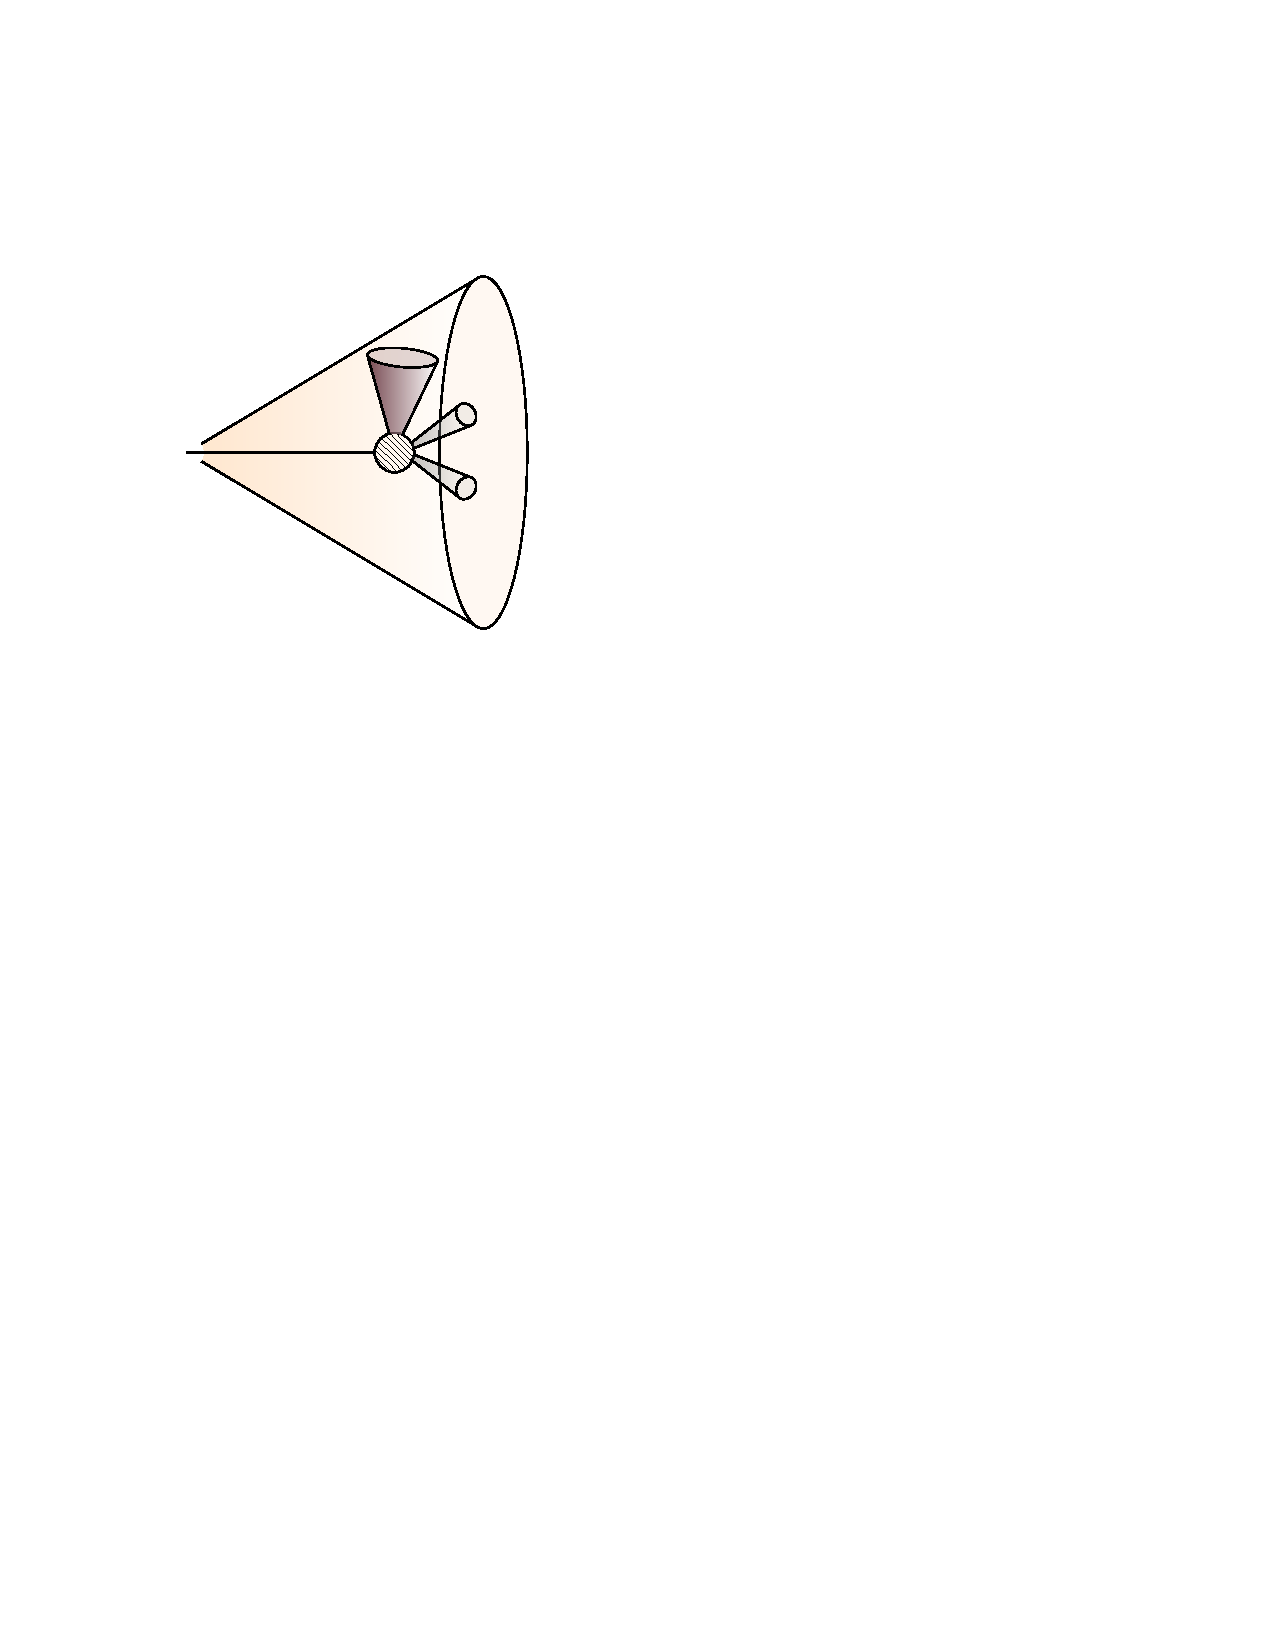
\includegraphics[width=.4\textwidth]{figures/misc/factorization/jet_fn_subjet_collinear_1.pdf}
%        \label{fig:shower:cartoon:subjet_collinear1}
%    }
%    \hfill
%    \subfloat[]{
%        % Subfigure graphic
%        \includegraphics[width=.4\textwidth]{example-image-a}
%        \label{fig:shower:cartoon:subjet_collinear2}
%    }

%    % Caption
%    \caption[Cartoons depicting the tools used in resummed EWOC computations]{
%    Depictions of the calculational tools involved in computations of (jet functions for) \hyperref[fig:shower:cartoon:subjet_collinear1]{(a)} generic two-point EWOCs, and \hyperref[fig:shower:cartoon:subjet_collinear2]{(b)} two-point EWOCs in the collinear limit.
%    %
%    The figure is nearly identical to the depiction of jet functions for the EEC in \Fig{shower:cartoon:collinear}, but uses subjets instead of particles.
%    %
%    \hyperref[fig:shower:cartoon:subjet_collinear1]{(a)} depicts the fragmentation of an initiating parton into a pair of final-state subjets, indicated by two small grey cones, and additional inclusive radiation indicated by a large red cone.
%    %
%    \hyperref[fig:shower:cartoon:subjet_collinear2]{(b)} visualizes a similar process in the collinear limit, in which the inclusive fragmentation of the initiating parton produces wide-angle radiation;
%    %
%    crucially, \hyperref[fig:shower:cartoon:subjet_collinear2]{(b)} depicts how the contributions to the EWOC in the collinear limit, which are nearly collinear final-state subjets, tend to emerge from the splitting of a single parton whose children then fragment into subjets.
%    %
%    The combination of partonic fragmentation and partonic splitting leads to a factorized expression for the EEC in the collinear limit, as in \Eq{eec_jet_fn_ll_1}.
%    \sam{ref in text?}
%    %
%    \sam{Need more fragmentation}
%    }

%    \label{fig:shower:cartoon:subjet_collinear}
%\end{figure}
%% -----------------------------------

%Similar arguments show that at LL, the subjet EEC within a jet initiated by a parton of type \(i\) is simply the corresponding particle-level EEC restricted to \(\chi > r^2 / 4\).
%%
%Expressing the EEC for such a jet as a jet function \(J^i(\chi, r; Q)\) as in \App{EEC:formal} and \Eq{eec_jet_fn_ll_1}, we write
%\begin{align}
%    J^i(\chi>0, r; Q)
%    &=
%    \frac{2 \as}{\chi}
%    \,
%    \Theta(\chi > r^2 /4)
%    \,
%    \sum_{ab}
%    \le(
%        \int_0^1 \dd z \, z (1-z) \,
%        P_{ab \leftarrow i}(z)
%    \ri)
%    \,
%    \le(
%        \frac{\alpha_s\le(2\,Q\sqrt{\chi}\ri)}
%        {\alpha_s\le(Q\,\Rjet\ri)}
%    \ri)
%    ^
%    {\frac{\hat{p}(m)}{2\pi\beta_0}}
%    _{f\leftarrow i}
%    .
%\end{align}



% ---------------------------------------
\Soln{The EEC in \texorpdfstring{\(e^+e^-\to\,\)}{ee to }hadrons}{ee_eec}
% ---------------------------------------

A more detailed description of the EEC at NLO in \(e^+e^-\to\,\)hadrons requires a treatment of the non-singular parts of the amplitude for \(e^+ e^- \to\,\)hadrons.
%
At NLO, the physics of \(e^+ e^- \to\,\)hadrons is captured by the process \(e^+ e^- \to q \overline{q} g\).
%
In terms of the variables \(x_i = 2 E_i / \sqrt{s} \in [0, 1]\), where \(i\,\in\,\{q,\overline{q},g\}\sim\,\{1,2,3\}\) denotes one of the three massless outgoing partons, the full differential cross section for \(e^+e^-\to q \overline{q} g\) is given by the well-known formula of \Eq{} \sam{do}
% TODO: e+e- to hadrons diff xsec with plus-fn
\begin{align}
    \dd \sigma
    =
    \sigma_0
    \,
    \ascf
    \,
    \dd x_i\,\dd x_j
    \,
    \frac{x_q^2 + x_{\overline{q}}^2}{
          {(1-x_q)}_+
          {(1-x_{\overline{q}})}_+
    }
    ,
\end{align}
where \(
    \sigma_0 =
    \frac{4\pi \alpha_{\text{EM}}^2}{3 s}
    \,N_c\,\sum_q \frac{e_q^2}{e^2}
\)
is the LO cross section for \(e^+e^-\to q \overline{q}\), summed over quark flavors with charges \(e_q\), and \(1/{(1-x)}_+\) denotes a \hyperlink{footnote:plusfn_defn}{\textit{plus-distribution}}.
%
The integration variables can be any pair \(x_i,\,x_j\) of \(x\)-variables with \(x_i\) ranging from 0 to 1 and \(x_j\) from 0 to \(1-x_i\);
%
the remaining variable is determined by the constraint \(x_q + x_{\overline{q}} + x_g = 2\).

In terms of the \(x_i\) the angle between partons \(i\) and \(j\) is given by
\begin{align}
    \cos\theta_{ij} = \frac{2}{x_i x_j} - \frac{2}{x_i} - \frac{2}{x_j} + 1
    \,,
\end{align}
as shown in \Prob{eetohadrons_kinematics}.

In terms of these variables, we may write the NLO EEC in integral form (away from \(\chi = 0\), if we neglect contact terms with \(i=j\)) as
\begin{align}
    \label{eq:ee2hadrons_EEC}
    \frac{\dd\Sigma_\text{EEC}}{\dd\chi}
    (\chi>0)
    =
    2
    \ascf
    \sum_{i<j}
    \int_0^1 \dd x_i
    &
    \int_{1-x_i}^1 \dd x_j
    \frac{x_q^2 + x_{\overline{q}}^2}{(1-x_q)_+(1-x_{\overline{q}})_+}
    \,\frac{x_i}{2}
    \,\frac{x_j}{2}
    \\
    &
    \notag
    \delta\le(
        \chi
        -
        \le(
            \frac{1}{x_i} + \frac{1}{x_j} - \frac{1}{x_i x_j}
        \ri)
    \ri)
    ,
\end{align}
where we have added an overall factor of \(2\) on the right-hand-side to write the sum over non-contact contributions as \(\sum_{i \neq j} = 2 \sum_{i < j}\), and we have used that \(E_i/Q = x_i / 2\).

The delta-function on the right-hand-side is activated when
\begin{align}
    x_j \to x_j^* \eqexclamation \frac{1-x_i}{1-\chi\,x_i}
    \,,
\end{align}
and its argument has Jacobian \(2(1 - \chi\,x_i)/(x_i x_j)\).

Using the delta-function, we may write the \(i\) and \(j\) dependent parts of the EEC integrand as
\begin{align}
    x_i\,x_j\,
    \delta\le(
        \frac{2}{x_i x_j} - \frac{2}{x_i} - \frac{2}{x_j} + 1
        -
        \cos\chi
    \ri)
    =
    \frac{1}{2}
    \frac{x_i^2\,x_j^2}{1 - z x_i}
    \delta(x_j - x_j^*)
    =
    \frac{1}{2}
    \frac{x_i^2\,(1-x_i)^2}{(1 - z x_i)^3}
    \delta(x_j - x_j^*)
    .
\end{align}
%
The EEC after the integration over \(x_j\) is then
\begin{align}
    \dv{\Sigma_\text{EEC}}{\cos\chi}{}
    &=
    \frac{\alpha_s C_F}{4\pi}
    \sum_{i<j}
    \int_0^1 \dd x_i\,
    x_i^2 (1 - x_i)^2
    \frac{1}{(1- z x_i)^3}
    \frac{x_1^2 + x_2^2}{(1-x_1)(1-x_2)}
    \Big|_{x_j = \frac{1-x_i}{1-z x_i}}
    \\
    &
    \eqdelta
    \frac{\alpha_s C_F}{4\pi}
    \sum_{i<j}
    {\mc J}_{ij}(z)
    \,,
\end{align}
where we have absorbed the integrals into the dimensionless functions \(\mc J_{ij}(z)\),
\begin{align}
    {\mc J}_{ij}(z)
    =
    \int_0^1 \dd x_i\,
    x_i^2 (1 - x_i)^2
    \frac{1}{(1- z x_i)^3}
    \frac{x_1^2 + x_2^2}{(1-x_1)(1-x_2)}
    \Big|_{x_j = \frac{1-x_i}{1-z x_i}}
    \label{eq:eec_integrals}
    \,.
\end{align}
%
We may therefore express \Eq{ee2hadrons_EEC} as the sum of simpler integrals for each \(i, j\) pair (\((i, j) = (1,2),\,(2,3)\).
%
We work these integrals out below, yielding the results
\begin{align}
    \mc J_{12}(\chi)
    &=
   \frac{1}{1-\chi}
   \le(
    \frac{-8}{\chi^4} + \frac{2}{\chi^3} + \frac{1/3}{\chi^2}
   \ri)
   +
   \frac{\log(1-\chi)}{1-\chi}
   \le(
    \frac{-8}{\chi^5} + \frac{6}{\chi^4}
   \ri)
    ,
\end{align}
and
\begin{align}
    \mc J_{13}(\chi)
    &=
    \frac{1}{1-\chi} \le(
        \frac{13}{\chi^4}
        -
        \frac{41/2}{\chi^3}
        +
        \frac{53/6}{\chi^2}
    \ri)
    +
    \log(1-\chi)\le(
        \frac{13}{\chi^5}
        +
        \frac{-14}{\chi^4}
        +
        \frac{4}{\chi^3}
    \ri)
    \,.
\end{align}

Consolidating gives the known result for the NLO EEC \cite{Basham:1978bw}
\begin{align}
    \label{eq:ee_to_hadrons_eec_nlo}
    \frac{\dd\Sigma_\text{EEC}}{\dd\chi}(\chi>0)
    &=
    \frac{\ascf}{2}
    \frac{3-2\chi}{(1-\chi)\chi^5}
    \le(
        3 \chi (2 - 3 \chi)
        +
        2 \log(1 - \chi) (2 \chi^2 - 6 \chi + 3)
    \ri)
    .
\end{align}
%
Notably, the collinear limit of the NLO result of \Eq{ee_to_hadrons_eec_nlo} contains exactly the universal feature we predicted in \Eq{universal_differential_eec},
\begin{align}
    \frac{\dd\Sigma_\text{EEC}}{\dd\chi}(\chi\to 0)
    &=
    \frac{3\ascf}{4\chi}
    +
    \mc O\le(\chi^0\ri)
    .
\end{align}
%
Furthermore, in the opposite limit -- associated with anti-collinear particle correlations with \(\theta = \pi\), we have
\begin{align}
    \frac{1}{\sigma_0}
    \dv{\Sigma_\text{EEC}}{\cos\chi}{}
    &\xrightarrow[\chi\to 1]{}
    \frac{\alpha_s C_F}{\pi}
    \le(
        \frac{1}{1-\chi}
        \le(
            -\log(1-\chi)
            -\frac{3}{2}
        \ri)
        - 5 \log(1-\chi)
    \ri)
    + \mc O\left((1-\chi)^0\right)
    \,.
\end{align}
%
Both singularities must be regularized in order to achieve the full EEC -- see \Prob{eec-dist}.



\vspace{7pt}
\hrule
\vspace{7pt}

Let us now evaluate the integrals.
%
By symmetry, \(\mc J_{13}(\chi) = \mc J_{23}(\chi)\), so we need only consider \(\mc J_{12}\) and \(\mc J_{13}\).
%
First, we notice that the \(x_1\) and \(x_2\) dependent part of the integrand must be considered separately for each case.

For \(\mc J_{12}\), we will use
\begin{align}
    i=1,&\,j=2:\notag
    \\
    \label{eq:constrained_integrand_12}
    &\frac{x_1^2 + x_2^2}{(1-x_1)(1-x_2)}
    \Big|_{x_2 = \frac{1-x_1}{1-\chi x_1}}
    =
    \frac{1}{1-\chi}\,
    \frac{1}{x_1}\,
    \frac{1}{1-x_1}\,
    \le(1 - \chi x_1\ri)
    \le(x_1^2 + \frac{1 - x_1}{1 - \chi x_1}\ri)^2
    \\
    &
    \qquad\qquad\qquad
    =
    \frac{1}{1-\chi}\,
    \frac{1}{x_1}\,
    \frac{1}{1-x_1}\,
    \frac{1}{1 - \chi x_1}\,
    \le(
        1 - 2 x_1 + 2 x_1^2 - 2 x_1^3 \chi + x_1^4 \chi^2
    \ri)
    \notag
    ,
\end{align}
where we have used that the constraint enforces
\begin{equation}
    1 - x_2
    \to
    1 - \frac{1-x_1}{1 - \chi x_1}
    =
    \frac{1 - \chi x_1 - 1 + x_1}{1 - \chi x_1}
    =
    x_1\frac{1-\chi}{1 - \chi x_1}
    .
\end{equation}

For \(\mc J_{13}\), we will use
%
\begin{align}
    i=1,&\,j=3:\notag
    \\
    \label{eq:constrained_integrand_13}
    &\frac{x_1^2 + x_2^2}{(1-x_1)(1-x_2)}
    \Big|_{x_3 = \frac{1-x_1}{1-\chi x_1}}
    =
    \frac{1}{\chi}\,
    \frac{1}{x_1}\,
    \le(\frac{1}{1-x_1}\ri)^2\,
    \le(1 - \chi x_1\ri)
    \le(
        x_1^2 + \le(1 - x_1 \chi \frac{1-x_1}{1 - \chi x_1}\ri)^2
    \ri)
    \\
    &
    \qquad\qquad
    =
    \frac{1}{\chi}\,
    \frac{1}{x_1}\,
    \le(\frac{1}{1-x_1}\ri)^2\,
    \frac{1}{1 - \chi x_1}\,
    \le(
        1 + x_1^2 - 4 x_1 \chi + 2 x_1^2 \chi - 2 x_1^3 \chi + 4 x_1^2 \chi^2 - 4 x_1^3 \chi^2 + 2 x_1^4 \chi^2
    \ri)
    \notag
    ,
\end{align}
where we have noticed \(
    x_1 + x_2 + x_3
    \to
    x_1 + x_2 + \frac{1-x_1}{1-\chi x_1}
    =
    2
\) from the constraint on \(x_3\), implying that \(x_2\) becomes
\begin{equation}
    x_2 \to 2 - x_1 - \frac{1-x_1}{1-\chi x_1}
    =
    1 - x_1 \le(
        1 - \frac{1-\chi}{1 - \chi x_1}
    \ri)
    =
    1 - x_1 \chi \frac{1-x_1}{1 - \chi x_1}
\end{equation}
and that \((1-x_2)\) therefore becomes
\begin{equation}
    1 - x_2
    \to
    \chi x_1 \frac{1 - x_1}{1 - \chi x_1}
    .
\end{equation}


Using \Eqs{constrained_integrand_12}{constrained_integrand_13} and performing the integrals in \texttt{Mathematica}, the \(\mc J_{ij}\) are then
\begin{align}
    \mc J_{12}(\chi)
    &=
    \int_0^1 \dd x_1\,
    x_1^2 (1 - x_1)^2
    \frac{1}{(1- \chi x_1)^3}
    \frac{x_1^2 + x_2^2}{(1-x_1)(1-x_2)}
    \Big|_{x_2 = \frac{1-x_1}{1-\chi x_1}}
    \\
    \notag
    &=
    \frac{1}{1-\chi}
    \int_0^1 \dd x_1\,
    x_1 (1 - x_1)
    \frac{1}{(1- \chi x_1)^4}
    \le(
        1 - 2 x_1 + 2 x_1^2 - 2 x_1^3 \chi + x_1^4 \chi^2
    \ri)
    \\
    &=
   \frac{1}{1-\chi}
   \le(
    \frac{-8}{\chi^4} + \frac{2}{\chi^3} + \frac{1/3}{\chi^2}
   \ri)
   +
   \frac{\log(1-\chi)}{1-\chi}
   \le(
    \frac{-8}{\chi^5} + \frac{6}{\chi^4}
   \ri)
    ,
\end{align}
and
\begin{align}
    \mc J_{13}(\chi)
    &=
    \notag
    \int_0^1 \dd x_1\,
    x_1^2 (1 - x_1)^2
    \frac{1}{(1- \chi x_1)^3}
    \frac{x_1^2 + x_2^2}{(1-x_2)}
    \Big|_{x_3 = \frac{1-x_1}{1-\chi x_1}}
    \\
    \notag
    &=
    \frac{1}{\chi}
    \int_0^1 \dd x_1\,
    x_1
    \frac{1}{(1- \chi x_1)^4}
    \le(
        1 + x_1^2 - 4 x_1 \chi + 2 x_1^2 \chi - 2 x_1^3 \chi + 4 x_1^2 \chi^2 - 4 x_1^3 \chi^2 + 2 x_1^4 \chi^2
    \ri)
    \\
    &=
    \frac{1}{1-\chi} \le(
        \frac{13}{\chi^4}
        -
        \frac{41/2}{\chi^3}
        +
        \frac{53/6}{\chi^2}
    \ri)
    +
    \log(1-\chi)\le(
        \frac{13}{\chi^5}
        +
        \frac{-14}{\chi^4}
        +
        \frac{4}{\chi^3}
    \ri)
    \,.
\end{align}
%
Again, by symmetry,
\begin{align}
    \mc J_{23}(\chi) &= \mc J_{13}(\chi).
\end{align}


% ---------------------------------------
\Soln{NLL Equivalence of New Angles}{nll_equiv}
% ---------------------------------------

We first emphasize that the parametrization we propose for PENCs only differs from the traditional PENCs studied in the literature through the jet function.
%
In particular, the factorization for our new parametrization is identical to that of the traditional PENCs in the collinear limit \cite{Dixon:2019uzg, Chen:2020vvp}:
\begin{align} \label{eq:fact}
    \Sigma_N
    \left(
    R_1, Q
    \right)
    =
    \int_0^1\!
    \dd x\,
    x^N
    \sum_i H_i
    \Bigl(x,\frac{Q}{\mu}\Bigr) \cdot
    J_i
    \Bigl( \frac{x^2 Q^2R_1^2}{\mu^2} \Bigr)
    \,,
\end{align}
where the flavor index \(i = q,g\)  is summed over.
%
At a specific perturbative order, the expressions also depend on $\mu$ through $\alpha_s(\mu)$.
%
%In particular,
\Eq{fact} states that the resummed cross section for the PENCs %jet observables should be
is governed by:
\begin{itemize}
    \item
    A \textit{hard function} \(H_i(x, Q/\mu)\), characterizing the number density of partons of partonic flavor \(i\) (e.g.\ up quark, gluon) emerging from the hard process at a given momentum fraction \(x\).
    %
    The hard function is dependent on a renormalization scale \(\mu\).
    %
    Notably, the hard function is independent of the parametrization used for the PENC.

    \item
    A \textit{jet function} \(J_i( x^2 Q^2R_1^2/\mu^2 )\), describing the subsequent evolution of the energetic parton \(i\)
    into a jet of ``final-state'' partons on which the PENC is then measured.
    %
    Unlike the hard function, the jet function depends on the parametrization of the observable.
\end{itemize}
%
In this appendix, we quantify the difference between the jet function for our new PENC (the \(R_1\) jet function) and the traditional PENC (the \(R_L\) jet function). Using theoretical arguments and numerical evidence, we argue that their difference is only relevant at next-to-next-to-leading-logarithmic (NNLL) order.

The resummation of logarithms of $R_1$ in $\Sigma_N$ can be achieved by evaluating the hard function at the scale $\mu_H \sim Q$ and the jet function at the scale $\mu_J \sim Q R_1$, and using the renormalization group equations to evolve them to a common scale $\mu$.
%
Since the full PENC is independent of \(\mu\), and the hard function is independent of the specific parametrization of the PENC, the renormalization group evolution for the jet function is also parametrization-independent (even if its functional form is not).

Within a jet consisting of two outgoing particles, the PENC we introduce and the traditional PENC are exactly the same, since \(R_1 = R_L\).
%
Therefore, the \(R_1\) jet function the \(R_L\) jet function are identical at \(\mathcal{O}(\alpha_s)\),
implying that the cross section for the new and traditional PENC will be equal at NLL, as these are single-logarithmic observables.
%
However, \(R_1\) and \(R_L\) will differ for a jet of three particles or more, corresponding to an ${\cal O}(\alpha_s^2)$ difference between the \(R_1\) and \(R_L\) jet functions, and an NNLL effect in the resummed cross section.


\begin{figure}[h]
    \centering
    	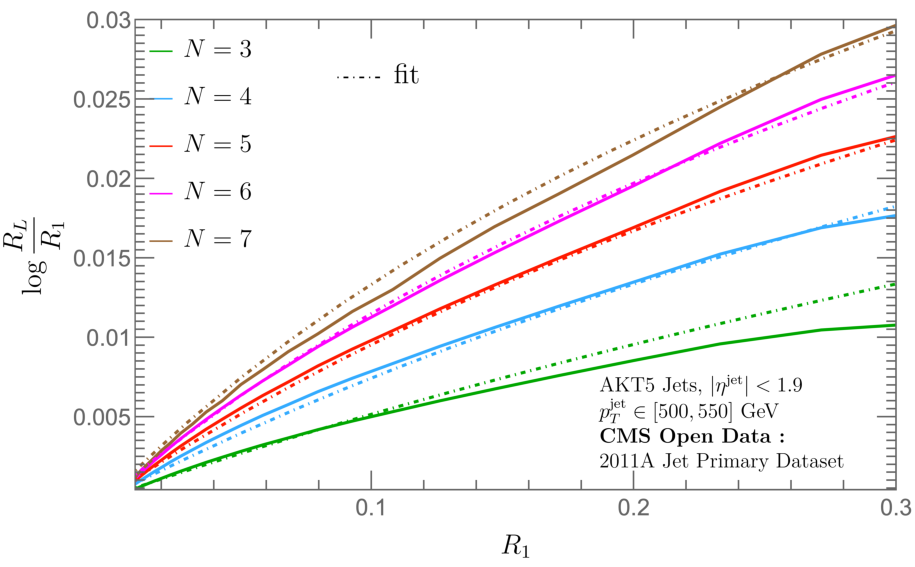
\includegraphics[width=0.6\textwidth]{figures/eec-angles/ENC_quantiles.pdf}
        \caption[Difference between the new and traditional parameterizations of projected energy correlators obtained from the quantiles of the corresponding cumulative distributions.]{
        Difference between the new parametrization ($R_1$) and the old parametrization ($R_L$) obtained from corresponding quantiles of the cumulative distributions.
        %
        The dashed lines correspond to a fit (of the overall coefficient) of the difference \( \log(R_L/R_1) \) to $\frac{\alpha_s}{\pi} \log(1+R_L\,(N-1))$ for integer values of $N$ from 3 to 7.
    }
	\label{fig:nll_equiv}%
\end{figure}


Though \(R_1\) and \(R_L\) differ in a generic jet, we note that $R_1 \leq R_L \leq 2R_1$ by the triangle inequality.
%
Therefore, we expect an approximate relationship between the two of the form $R_L \sim (1+c) R_1$ with $0<c<1$.
%
Furthermore, NLL equivalence of the \(R_1\) and \(R_L\) jet functions implies that  $c \sim {\cal O}(\alpha_s)$.
%
In particular,
writing the N\(^k\)LL contribution to the traditional PENC as $\sum_{n} d_{n,k}\alpha_s^{n+k}\log^n R_L$
and inserting $R_L = (1+c) R_1$ yields:
\begin{align}
    \label{eq:c_is_alphas}
   \sum_{n,k}
       d_{n,k} \alpha_s^{n+k}
       \log^n[
           R_1
           (1 +
           c)
       ]
   &=
   \sum_{n,k}
      d_{n,k} \alpha_s^{n+k}[\log R_1 +\log(1+c)]^n
  \nn \\
   &=
   \sum_{m,k,k'}
      {m+k' \choose m}
      d_{m+k', k} \alpha_s^{m+k+k'} \log^m R_1 \log^{k'} (1+c)
      \,,
\end{align}
where in the final line we have written \(n = m + k'\).
%
The terms with \(k' = 0\) give precisely the traditional PENC but with the argument \(R_L\) replaced by \(R_1\).
%
For \(k' = 1\) this would represent an NLL effect. However, the difference between our new PENC and the traditional PENC starts at NNLL, implying that $\log(1+c) \sim {\cal O}(\alpha_s)$ and thus $c \sim {\cal O}(\alpha_s)$.


Finally, we present additional numerical evidence that \(R_L \sim \left(1+c\right)R_1\) with \(c \sim \mathcal{O}(\alpha_s)\) by using the cumulative distributions for \(R_1\) and \(R_L\) to construct a correspondence between $R_1$ and $R_L$ using quantiles~\cite{Brewer:2018dfs}.
%
In particular, we numerically invert the equation
\begin{align}
   \label{eq:quantiles}
   \Sigma^\text{new}_{N}(R_1)
   =
   \Sigma^\text{old}_N(
       R_L
       %=
       %(1 +\mathcal{O}(\alpha_s))
       (R_1)
   )
   \, ,
\end{align}
to find a functional form for \(R_L(R_1)\).
%
In words, \Eq{quantiles} selects a function \(R_L(R_1)\) for which our new PENC and the traditional PENC have equivalent cumulative distributions.
%
\Fig{nll_equiv} displays the difference between $\log(R_L(R_1))$ and $\log R_1$, as a function of $R_1$, for $N=$ 3, 4, 5, 6, and 7.
%
The dashed lines correspond to a fit (of the overall constant) to the form $c \sim \alpha_s/\pi\, \log[1+(N-1) R_L]$.
%
This provides numerical evidence for our theoretical arguments that the \(R_1\) and \(R_L\) jet functions are equivalent at NLL, and that $R_L = [1 + {\mathcal O}(\alpha_s)] R_1$.

\vspace{15pt}


% ---------------------------------------
\Soln{Implementing New Angles for Energy Correlators}{eec-angles_pseudocode}
% ---------------------------------------

\begin{table}%[ht!]
\hspace{-60pt}
% \makebox[1.4 \textwidth][c]{ %to center table
% \resizebox{1.4 \textwidth}{!}{ %to resize table
\begin{minipage}{0.58\textwidth}
\hrule height 1.3pt
\vspace{4pt}
{
    \hypertarget{alg:penc}{ALG I.}\,
    \textbf{Pseudocode} for PENC($R_1$)
}
\vspace{4pt}
\hrule
\hrule
\vspace{5pt}
\begin{algorithmic}[1]
    \State \textbf{Output:} Normalized 1-dimensional histogram
    \State \qquad\qquad\,{}
    containing the PENC
    \\
    \State
    \textbf{Initialize} 1D $histogram$ to contain the PENC
    \State \textcolor{codegreen!80!black}{\# Loop over jets in a sample:}
    \ForAll{$i$ \textbf{from} $1$ \textbf{to} $n\_jets$}
        \State $jet \gets$ a jet from the desired sample
        \State \textcolor{codegreen!80!black}{\# Loop over choices for particle $s$ in the jet:}
        \ForAll{particles $s$ in $jet$}
            \State \textcolor{codegreen!80!black}{\# Calculate energy weight}
            \State $z_s \gets $ \(p_{T,\, s}/(\sum_j p_{T,\,j})\)
            \State \textbf{Sort} particles in $jet$ by angle to $s$,
            \State
            \qquad\,\,from \textit{smallest to largest}
            \State \textcolor{codegreen!80!black}{\# Prepare to record total weight within a}
            \State \textcolor{codegreen!80!black}{\# distance \(R_1\) of \(s\), beginning with \(R_1=0\)}
            \State \textbf{Initialize} $sum\_z_1 \gets z_s$
                \State
                $histogram[0]$
                +=
                $z_s^N$
            \State \textcolor{codegreen!80!black}{\# Loop over remaining particles $i_1$}
            \ForAll {$i_1$ \textbf{from} $1$ \textbf{to} len(particles)}
                \State $R_1 \gets$ angle between $s$ and particle[$i_1$]
                \State $z_1 \gets $ \(p_{T,\, i_1}/(\sum_j p_{T,\,j})\)
                \State \textcolor{codegreen!80!black}{\# Calculate contribution to $\dd\Sigma$, and}
                \State \textcolor{codegreen!80!black}{\# update hist. bin for $R_1$}
                \State
                $histogram[R_1]$
                +=
                $z_s
                \,\,\,\,
                \times $
                \\
                \qquad\qquad\qquad\quad
                $\bigl(
                    (
                        sum\_z_1 + z_1
                    )^{N-1}
                    -
                    sum\_z_1^{N-1}
                \bigr)
                $
                \State
                \textcolor{codegreen!80!black}{\# Update sum on weights within \(R_1\)}
                \State
                $sum\_z_1 +\!\!= z_1$
            \EndFor
        \EndFor
    \EndFor
    \\
    \State \textcolor{codegreen!80!black}{\# $histogram$ now contains $\dd\Sigma$, and we want}
    \State \textcolor{codegreen!80!black}{\# PENC$\,=\dd \Sigma/\dd R_1$}
    \State \textbf{Process} $histogram$ into a probability density by
    \\
    \qquad\qquad\,normalizing it relative to bin widths
    \State \textbf{Write} $histogram$ to output file
\end{algorithmic}
\vspace{5pt}
\hrule height 1.3pt
\end{minipage}
%
\hspace{10pt}
\vline
\hspace{10pt}
%
\begin{minipage}{0.58\textwidth}
\hrule height 1.3pt
\vspace{4pt}
{
    \hypertarget{alg:re3c}{ALG II.}\, %\quad{}
    \textbf{Pseudocode} for RE3C($R_1,R_2,\phi_2$)
}
\vspace{4pt}
\hrule
\hrule
\vspace{5pt}
\begin{algorithmic}[1]
    \State \textbf{Output:} Normalized 3-dimensional histogram
    \State \qquad\qquad\,{}
    containing the RE3C
    \\
    \State
    \textbf{Initialize} 3D $histogram$ to contain the RE3C
    \State \textcolor{codegreen!80!black}{\# Loop over jets in a sample:}
    \ForAll{$i$ \textbf{from} $1$ \textbf{to} $n\_jets$}
        \State $jet \gets$ a jet from the desired sample
        \State \textcolor{codegreen!80!black}{\# Loop over choices for particle $s$ in the jet:}
        \ForAll{particles $s$ in $jet$}
            \State \textcolor{codegreen!80!black}{\# Calculate energy weight}
            \State $z_s \gets $ \(p_{T,\, s}/(\sum_j p_{T,\,j})\)
            \State \textbf{Sort} particles in $jet$ by angle to $s$,
            \State
            \qquad\,\,from \textit{smallest to largest}
            \State \textcolor{codegreen!80!black}{\# Loop over remaining particles $i_1$ and $i_2$,}
            \ForAll {$i_1$ \textbf{from} $1$ \textbf{to} length(particles)}
                \State $R_1 \gets$ angle between $s$ and particle[$i_1$]
                \State $z_1 \gets $ \(p_{T,\, i_1}/(\sum_j p_{T,\,j})\)
                \State \textcolor{codegreen!80!black}{\# where $i_2$ is \textit{closer} to $s$ than $i_1$}
                \ForAll {$i_2 < i_1$}
                    \State $R_2 \gets$ angle between $s$ and $i_2$
                    \State $z_2 \gets $ \(p_{T,\, i_2}/(\sum_j p_{T,\,j})\)
                    \State $\phi_2 \gets $ angle associated with $i_1$-$s$-$i_2$
                    \State \textcolor{codegreen!80!black}{\# Calculate contribution to $\dd\Sigma$,}
                    \State \textcolor{codegreen!80!black}{\# and update associated hist. bin}
                    \State
                    $histogram[R_1][R_2][\phi_2]$
                    +=
                    $z_s \cdot z_1 \cdot z_2$
                \EndFor
            \EndFor
        \EndFor
    \EndFor
    \\
    \State \textcolor{codegreen!80!black}{\# $histogram$ now contains $\dd\Sigma$, and we want}
    \State \textcolor{codegreen!80!black}{\# RE3C$\,=\dd \Sigma/\dd R_1 \dd R_2 \dd \phi_2$}
    \State \textbf{Process} $histogram$ into a probability density by
    \\
    \qquad\qquad\,normalizing it relative to bin widths
    \State \textbf{Write} $histogram$ to output file
\end{algorithmic}
\vspace{8pt}
\hrule height 1.3pt
\end{minipage}
% } %close resize
% } %close table
\end{table}

\vspace{10pt}

We provide pseudocode of our new algorithms for calculating PENCs and RE3Cs in Algs.~\hyperlink{alg:penc}{I} and  \hyperlink{alg:re3c}{II}, respectively.
%
Alg.~\hyperlink{alg:penc}{I} exemplifies how the parametrization we introduce for the PENC (i.e.~of angles with respect to a specific particle $s$) simplifies the $N$-dependence of our new PENC, and dramatically speeding up  the associated computation.
%
In particular, \emph{there are no additional computational complications for large or non-integer \(N\).}
%
For completeness, we also present pseudocode for the RE3C in Alg. \hyperlink{alg:re3c}{II}, which features similar computational simplicity and can be easily generalized to a double-projected ENC as discussed in the main text.
%
For a more complete and technical description of each computation, including permutation factors and contact terms, please consult our implementation available on GitHub at \texttt{ResolvedEnergyCorrelators}~\cite{github:RENC}.


% ---------------------------------------
\Soln{Non-Perturbative Features of Resolved Energy Correlators}{enc-nonpert}
% ---------------------------------------


Finally, we investigate the non-perturbative features of the new RENCs we introduce in this work, focusing on the example provided by the density plots for the \(\phi_2\)-integrated RE3C which we visualize again in \Fig{nonpert}.
%
For notational convenience in the discussion below, we let $p_T$ be shorthand for $p_T^\text{jet}$.
%
Unlike in the traditional E3C, for which there are only non-perturbative effects in the squeezed configuration with \(R_S \sim \Lambda_\text{QCD}/p_T\), our new RE3C exhibits non-perturbative features in two regimes:  (1) when \(R_2 \sim \Lambda_\text{QCD}/p_T\), when particle \(i_2\) (the emission that sets \(R_2\)) approaches the special particle \(s\); and (2) when \(R_1 - R_2 \sim \Lambda_\text{QCD}/p_T\), with the possibility that \(i_2\) approaches \(i_1\).

However, the shapes of the non-perturbative features of the integrated RE3C of \Fig{nonpert_density} are not exactly symmetric under a reflection about the line \(R_2 = R_1/2\):
%
the ridge in \Fig{nonpert_density} when \(R_2 \to R_1\) has a smaller slope than the ridge when \(R_2 \to 0\).
%
Concretely, this means that \(R_2\) must get closer to \(R_1\) in order for non-perturbative features to emerge than we might naively expect.
%
We refer to this as the ``\(R_2\)-asymmetry'' of the integrated RE3C.

To explain this \(R_2\)-asymmetry, we note that when $R_2 \sim \Lambda_{\rm QCD}/p_T$, shown by the dashed yellow line in \Fig{nonpert}\,, the particle $i_2$ is non-perturbatively close to \(s\), independent of the orientation $\phi_2$ of particle $i_2$ around $s$.
%
On the other hand, when \(R_2 \sim R_1 - \Lambda_\text{QCD}/p_T\), particle \(i_2\) is not guaranteed to be near \(i_1\).
%
Instead, \(i_2\) is only non-perturbatively close to \(i_1\) in a narrow range of azimuthal angles centered around \(\phi_2 = 0\), as visualized in \Fig{nonpert_cartoon}.
%
Therefore, it is only when \(R_2\) gets significantly closer to \(R_1\) that the non-perturbative features of the integrated RE3C begin to emerge.


\begin{figure}[t]
    \centering
    \subfloat[]{
    	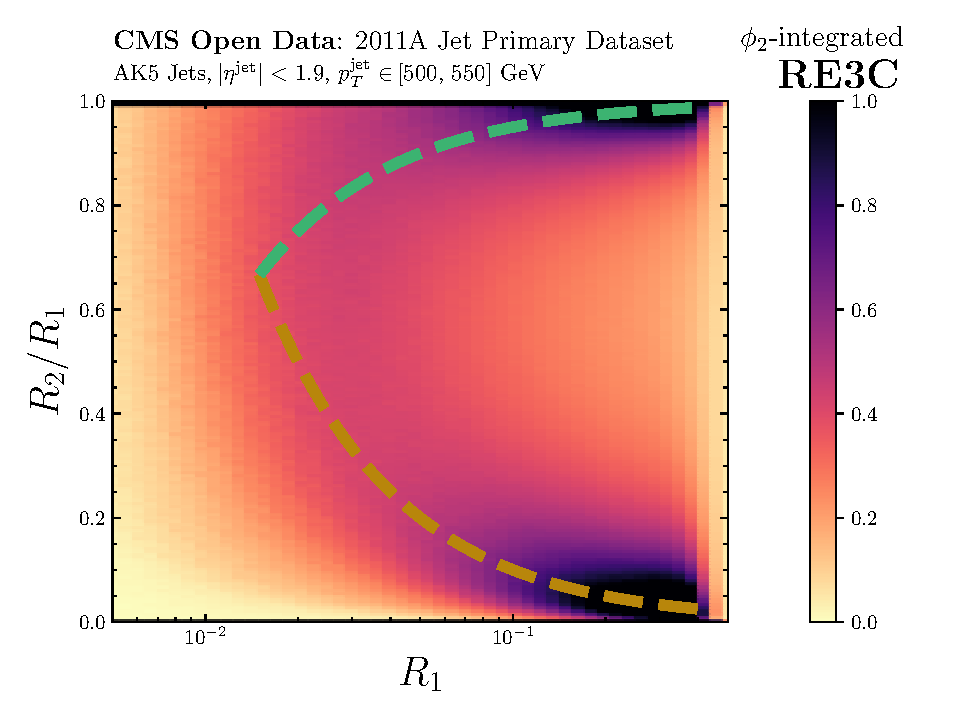
\includegraphics[width=0.5\textwidth]{figures/eec-angles/opendata/od_nonpert_density.pdf}
    	\label{fig:nonpert_density}
    }
    \subfloat[]{
        \begingroup
        \tikzset{every picture/.style={scale=1.3}}%
        	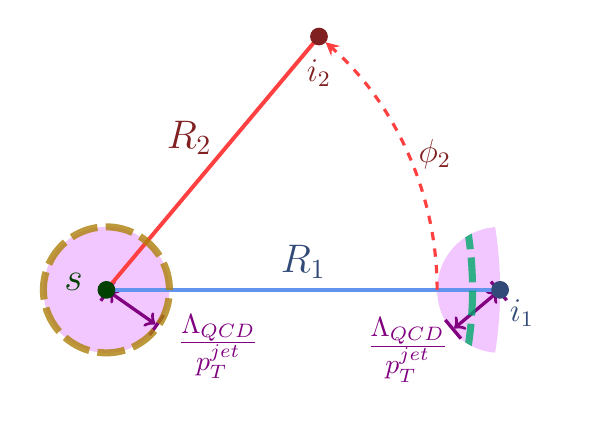
\begin{tikzpicture}
% Defining colors 
\definecolor{cornflowerblue}{rgb}{0.39, 0.58, 0.93}
\definecolor{azure(colorwheel)}{rgb}{0.0, 0.5, 1.0}

\definecolor{coralred}{rgb}{1.0, 0.25, 0.25}
\definecolor{cadmiumorange}{rgb}{0.93, 0.53, 0.18}
\definecolor{darkgoldenrod}{rgb}{0.72, 0.53, 0.04}
\definecolor{pastelorange}{rgb}{1.0, 0.7, 0.28}

\definecolor{rosevale}{rgb}{0.67, 0.31, 0.32}
\definecolor{palebrown}{rgb}{0.6, 0.46, 0.33}
\definecolor{goldenpoppy}{rgb}{0.99, 0.76, 0.0}
\definecolor{gold(metallic)}{rgb}{0.83, 0.69, 0.22}

\definecolor{heliotrope}{rgb}{0.87, 0.45, 1.0}
\definecolor{mediumorchid}{rgb}{0.73, 0.33, 0.83}

\definecolor{ao}{rgb}{0.0, 0.5, 0.0}
\definecolor{lightseagreen}{rgb}{0.13, 0.7, 0.67}
\definecolor{jade}{rgb}{0.0, 0.66, 0.42}

% Defining colors associated with different nodes
\colorlet{colsp}{ao}
\colorlet{coli1}{cornflowerblue}
\colorlet{coli2}{coralred}

% All grey
% \colorlet{colsp}{gray}
% \colorlet{coli1}{gray}
% \colorlet{coli2}{gray}
% \colorlet{coli3}{gray}
% \colorlet{coliN}{gray}


% Nonperturbative Regions
\begin{scope}
    % Clip
    \clip(-1,-1.5) rectangle (5,2);
    \clip (0, 0) circle (5);

    % Circles around s and i1
    \fill[heliotrope, opacity=0.4] (5, 0) circle (0.8);
    \fill[heliotrope, opacity=0.4] (0, 0) circle (0.8);

    % Lambda_QCD indication
    \coordinate (O1) at (0, 0);
    \coordinate (E1) at (-35:0.8);
    \draw[|<->|,blue!50!red, very thick] (O1)--(E1)
    node[pos=0.8, right, yshift=-10pt, xshift=7pt, font=\Large]
    {\textcolor{blue!50!red}{$\frac{\Lambda_\text{QCD}}{p_T^\text{jet}}$}};
\end{scope}
\begin{scope}[xshift=5cm]
    \coordinate (O1) at (0, 0);
    \coordinate (E1) at (-140:0.8);
    \draw[|<->|,blue!50!red, very thick] (O1)--(E1)
    node[pos=0.8, right, yshift=-10pt, xshift=-38pt, font=\Large]
    {\textcolor{blue!50!red}{$\frac{\Lambda_\text{QCD}}{p_T^\text{jet}}$}};
\end{scope}

% =:=:=:=:=:=:=:=:=:=:=:=:=:=:=:=:=:=:=
% Particle 1
% =:=:=:=:=:=:=:=:=:=:=:=:=:=:=:=:=:=:=
\draw[color=coli1, line width=0.5mm] 
    (0, 0) -- (0:5) coordinate (i1)
    node[pos=0.5, above, sloped, text=black,
         font=\Large]
        {\textcolor{coli1!50!black}{$\boldsymbol{R_1}$}};
    
% i1 node
\filldraw[color=coli1!50!black] 
    (i1) circle (3pt) 
    node[below right, font=\large]
    {\textcolor{coli1!50!black}{$i_1$}};

% =:=:=:=:=:=:=:=:=:=:=:=:=:=:=:=:=:=:=
% Particle 2
% =:=:=:=:=:=:=:=:=:=:=:=:=:=:=:=:=:=:=
\draw[color=coli2, line width=0.5mm]
    (0, 0) -- (50:4.2) coordinate (i2)
    node[pos=0.6, left, text=black, xshift=-4pt, font=\Large]
    {\textcolor{coli2!50!black}{$\boldsymbol{R_2}$}};

% phi_2 arc
\draw[-stealth, color=coli2, dashed, line width=0.4mm] 
    (0:4.2) 
    arc [start angle=0, end angle=48.5, radius=4.2]
    node[pos=0.5, right, text=black, font=\large]
    {\textcolor{coli2!50!black}{$\phi_2$}};

% i2 node
\filldraw[coli2!50!black] 
    (i2) circle (3pt)
    node[below, yshift=-5pt, font=\large]
    {\textcolor{coli2!50!black}{$i_2$}};


% =:=:=:=:=:=:=:=:=:=:=:=:=:=:=:=:=:=:=
% Draw the central point s
% =:=:=:=:=:=:=:=:=:=:=:=:=:=:=:=:=:=:=
\filldraw[color=colsp!50!black]
    (0, 0) circle (3pt) 
    node[left, yshift=3pt, xshift=-5pt, font=\Large]
    {\textcolor{colsp!50!black}{$s$}};


% =:=:=:=:=:=:=:=:=:=:=:=:=:=:=:=:=:=:=
% Non-perturbative phase space
% =:=:=:=:=:=:=:=:=:=:=:=:=:=:=:=:=:=:=
\begin{scope}
    \clip (5, 0) circle (0.8);
    \draw[color=jade, 
    dash pattern=on 9pt off 3pt,
    line width=0.9mm, opacity=0.8] 
    (-30:4.65) 
    arc [start angle=-30, end angle=30, radius=4.65];
\end{scope}

\begin{scope}
    \draw[color=darkgoldenrod!95!black,
    dash pattern=on 10pt off 3pt,
    line width=0.9mm, opacity=0.8] (0, 0) circle (0.8);
\end{scope}

\end{tikzpicture}
        \endgroup
    	\label{fig:nonpert_cartoon}
    }
    \caption[Non-perturbative features of the resolved three-point energy correlator.]{
        Depictions of the non-perturbative features of the RE3C introduced in this work \textbf{(a)} highlighted in a two-dimensional density plot, and \textbf{(b)} in a simple cartoon demonstrating the relevant non-perturbative regimes.
        %
        \textbf{(a)}
        A density plot for the RE3C evaluated on CMS Open Data and integrated over \(\phi_2\), taken from Fig.~4 of the main text, together with dashed lines indicating where non-perturbative effects are expected to become important using (geometric) phase space considerations.
        %
        \textbf{(b)}
        The RE3C geometry, with non-perturbative regions of phase space highlighted in purple, and with the dashed lines near \(s\) and \(i_2\) indicating the values of \(R_2\) where we expect non-perturbative features to emerge in the integrated RE3C.
    }
	\label{fig:nonpert}
\end{figure}

We estimate the \(R_2\)-asymmetry of the integrated RE3C by noting that non-perturbative features emerge when the measure of the non-perturbative phase space for \(i_2\) near \(i_1\) is comparable to the non-perturbative phase space for \(i_2\) near \(s\).
%
This is visualized in \Fig{nonpert_cartoon}:
%
non-perturbative features of the integrated RE3C emerge when the length of the green dashed line near \(i_1\) has a length of order \(\Lambda_\text{QCD}/p_T\).
%
The associated geometric constraint is a complicated solution to a cubic equation and we do not show it here.
%
However, we show our resulting estimate of the non-perturbative features as the green dashed line in \Fig{nonpert_density}, which aligns closely with the non-perturbative ridge of the integrated RE3C as \(R_2\) approaches \(R_1\).



% ---------------------------------------
\Soln{A Would-Be Particle-Level EWOC}{ee_ewoc}
% ---------------------------------------

The setup of this problem is identical to that of \Prob{ee_eec};
%
the phase space is identical, and only the argument of the delta function is different.
%
Recalling that \(m^2_{ij} / Q^2 = x_i + x_j - 1\) from \Prob{eetohadrons_kinematics}, we may write the NLO, would-be particle-level mass EWOC in integral form (away from \(\chi = 0\), if we neglect contact terms with \(i=j\)) as
\begin{align}
    \label{eq:ee2hadrons_EEC}
    \frac{\dd\Sigma_{m^2}}{\dd\chi}
    (\chi>0)
    =
    \frac{2\ascf}{Q^2}
    \sum_{i<j}
    \int_0^1 \dd x_i
    &
    \int_{1-x_i}^1 \dd x_j
    \frac{x_q^2 + x_{\overline{q}}^2}{(1-x_q)_+(1-x_{\overline{q}})_+}
    \,\frac{x_i}{2}
    \,\frac{x_j}{2}
    \\
    &
    \notag
    \delta\le(
        \chi +
        1 - x_i - x_j
    \ri)
    \,,
\end{align}
where we have added an overall factor of \(2\) on the right-hand-side to write the sum over non-contact contributions as \(\sum_{i \neq j} = 2 \sum_{i < j}\), and we have used that \(E_i/Q = x_i / 2\).


    Answer related to IRC safety only being a problem with three or more emissions


% ---------------------------------------
\Soln{Numerically Resummed EWOCs}{resummed-ewoc}
% ---------------------------------------

I began implementing code for DGLAP evolution of \gls{parton-to-parton} in the \texttt{plot/qcd/fragmentation.py} in \texttt{ResolvedEnergyCorrelators}~\cite{github:RENC}, but was unable to get my results to agree with existing results for microjet fragmentation \cite{Dasgupta:2014yra,Dasgupta:2016bnd} (my code for comparing the two is at \texttt{plot/fragmentation/inclusive\_microjets.py}).
%
I welcome you to look at, borrow, or steal my code!
%
This is probably a neat paper once the computational tools are properly set up.





\iffalse
% ==============================================
\section*{Appendices}
% ==============================================


% ---------------------------------------
\Soln{The Cauchy Principle Value}{principle-value}
% ---------------------------------------
Luckily, distributions are quite amenable to formal manipulations, and we present a formal (though not quite rigorous) proof below.
%
We can use
\begin{align}
    \abs{x}
    =
    x\le(\Theta(x)-\Theta(-x)\ri)
    \,,
\end{align}
so that
\begin{align}
    \dv{\abs{x}}{x}
    =
    \le(\Theta(x)-\Theta(-x)\ri)
    +
    2 x \delta(x)
    =
    \Theta(x)-\Theta(-x)
    \,,
\end{align}
and therefore
\begin{align}
    \dv{\ln(\abs{x})}{x}
    =
    \frac{1}{\abs{x}}\dv{\abs{x}}{x}
    =
    \frac{1}{\abs{x}}
    \le(
        \Theta(x)-\Theta(-x)
    \ri)
    \,,
\end{align}
from which we can immediately write, at least formally, that
\begin{align}
    \int_{-\infty}^\infty
    \,
    \dv{\ln(\abs{x})}{x}
    \,
    \phi(x)
    \,
    \dd x
    =
    \int_0^\infty
    \,
    \dd x
    \,\,
    \frac{\phi(x) - \phi(-x)}{x}
    \,.
\end{align}





% ---------------------------------------
\Soln{The Sokhatski-Plemelj Formula}{sokhatski-plemelj}
% ---------------------------------------
Since \(\log(z) = \log(|z|) + i \arg{z}\) for complex \(z\), we have
\begin{align}
    \lim_{\epsilon \to 0}
    \log(x \pm i \epsilon)
    =
    \log(\abs{x}) \pm i \pi \Theta(x < 0)
    \,.
\end{align}
for real \(x\).
%
Taking derivatives and using the result of the previous problem yields
\begin{align}
    \frac{1}{x \pm i \epsilon}
    =
    \text{PV}\le(\frac{1}{x}\ri)
    \mp
    i\pi \delta(x)
    \,.
\end{align}




% ---------------------------------------
\Soln{Two Plus, One Delta}{two-plus_one-delta}
% ---------------------------------------
A distribution proof of this claim is possible, but somewhat lengthy.
%
Instead, let us first notice that integrating this against \(\dd b\,g(b)\) gives
\begin{align}
    \int_0^2 \dd b\,g(b)
    \int_{0}^{1} \dd x\,
    \int_{1-x}^{1} \dd y\,
    &
    \le[\frac{1}{1-x}\ri]_+
    \le[\frac{1}{1-y}\ri]_+
    \delta(b - x - y)
    \notag
    \\
    &=
    \notag
    \int_{0}^{1} \dd x\,
    \int_{1-x}^{1} \dd y\,
    \le[\frac{1}{1-x}\ri]_+
    \le[\frac{1}{1-y}\ri]_+
    g(x + y)
    \\
    &=
    \notag
    \int_{0}^{1} \dd x\,
    \le[\frac{1}{1-x}\ri]_+
    \le(
        \int_{1-x}^{1} \dd y\,
        \frac{g(x + y) - g(x + 1)}{1-y}
        -
        \int_0^{1-x} \dd y\,
        \frac{g(x + 1)}{1-y}
    \ri)
    \\
    &=
    \int_{0}^{1} \dd x\,
    \frac{1}{1-x}
    \Bigg(
        \int_{1-x}^{1} \dd y\,
        \frac{g(x + y) - g(x + 1)}{1-y}
    \notag
        \\
        &\qquad\qquad\qquad\qquad
        -
        \int_{0}^{1} \dd y\,
        \frac{g(1 + y) - g(2)}{1-y}
    \label{eq:two-plus_one-delta_distribution}
        \\
    \notag
        &\qquad\qquad\qquad\qquad
        -
        \int_0^{1-x} \dd y\,
        \frac{g(x + 1)}{1-y}
    \Bigg)
    .
\end{align}
%
In going to the second line, we have performed the integral over \(b\) to eliminate the delta-function.
%
In going to the third line, we have used the definition of the plus-distribution to write the integral over \(y\) in terms of actual functions.
%
In going to the fourth line, we have similarly expanded the integral over \(x\).

This is sufficiently general that any consistent definition of \Eq{two-plus_one-delta} should be equivalent to this one.
%
Note, for example, that it gives the expected answer of \(\zeta(2)\) for the case \(g(b) = 1\).


One approach to evaluating this integral is to use the delta-function identity we have already seen:
\begin{align}
    \int_{0}^{1} \dd x\,
    \int_{1-x}^{1} \dd y\,
    \le[\frac{1}{1-x}\ri]_+
    \le[\frac{1}{1-y}\ri]_+
    \delta(b - x - y)
    &=
    \Theta(b > 1)
    \int_{b-1}^{1} \dd x\,
    \le[\frac{1}{1 - x}\ri]_+
    \le[\frac{1}{1 + x - b}\ri]_+^{x\in(b-1,1)}
    ,
\end{align}
where we have used the result of \Eq{mixed-bounds_1d_plus-distribution}:
\begin{align}
    \int_{1-x}^{1} \dd y\,
    \le[\frac{1}{1-y}\ri]_+
    \delta(b - x - y)
    &=
    \le[\frac{1}{1 + x - b}\ri]_+^{x\in(b-1,b)}
    \Theta(x > b - 1)\Theta(b > 1)
    .
\end{align}

It is not immediately clear how we should proceed.
%
Let us attempt to divide the integral into two parts:
\begin{align}
    \int_{b-1}^{1} \dd x\,
    \le[\frac{1}{1 - x}\ri]_+
    \le[\frac{1}{1 + x - b}\ri]_+^{x\in(b-1,b)}
    &=
    \int_{b-1}^{a} \dd x\,
    \le[\frac{1}{1 - x}\ri]_+
    \le[\frac{1}{1 + x - b}\ri]_+^{x\in(b-1,b)}
    \label{eq:double_plus}
    \\
    &~~~~+
    \int_{a}^{1} \dd x\,
    \le[\frac{1}{1 - x}\ri]_+
    \le[\frac{1}{1 + x - b}\ri]_+^{x\in(b-1,b)}
    \notag
    ,
\end{align}
where \(a\) is some intermediate value between \(b-1\) and \(1\), and we will leave the factor of \(\Theta(b > 1)\) implicit until the end of our discussion.

The first integral -- the one on the first line of \Eq{double_plus} -- gives
\begin{align}
    \int_{b-1}^{a} \dd x\,
    \le[\frac{1}{1 - x}\ri]_+
    \le[\frac{1}{1 + x - b}\ri]_+^{x\in(b-1,b)}
    &=
    \int_{b-1}^{a} \dd x\,
    \frac{1}{1 - x}
    \le[\frac{1}{1 + x - b}\ri]_+^{x\in(b-1,b)}
    \\
    &=
    \int_{b-1}^{a} \dd x\,
    \le(
        \frac{1}{1 - x} - \frac{1}{2 - b}
    \ri)
    \frac{1}{1 + x - b}
    \notag
    \\
    &~~~~-
    \int_{a}^{b} \dd x\,
    \frac{1}{2 - b}
    \frac{1}{1 + x - b}
    \\
    &=
    \frac{\log(2-b) - \log(1-a)}{2 - b}
    +
    \frac{\log(1+a-b)}{2 - b}
    \notag
    .
\end{align}

The second integral -- the one on the second line of \Eq{double_plus} -- gives
\begin{align}
    \int_{a}^{1} \dd x\,
    \le[\frac{1}{1 - x}\ri]_+
    \le[\frac{1}{1 + x - b}\ri]_+^{x\in(b-1,1)}
    &=
    \int_{a}^{1} \dd x\,
    \le[\frac{1}{1 - x}\ri]_+
    \frac{1}{1 + x - b}
    \\
    &=
    \int_{a}^{1} \dd x\,
    \frac{1}{1 - x}
    \le(
        \frac{1}{1 + x - b} - \frac{1}{2 - b}
    \ri)
    \notag
    \\
    &~~~~-
    \int_{0}^{a} \dd x\,
    \frac{1}{2 - b}
    \frac{1}{1 - x}
    \\
    &=
    \frac{\log(2-b) - \log(1+a-b)}{2 - b} + \frac{\log(1-a)}{2 - b}
    \notag
    .
\end{align}

Summing these and adding back the factor of \(\Theta(b-1)\), we appear to get
\begin{align}
    \int_{0}^{1} \dd x\,
    \int_{1-x}^{1} \dd y\,
    \le[\frac{1}{1-x}\ri]_+
    \le[\frac{1}{1-y}\ri]_+
    \delta(b - x - y)
    &=
    \Theta(b > 1)
    \int_{b-1}^{1} \dd x\,
    \le[\frac{1}{1 - x}\ri]_+
    \le[\frac{1}{1 + x - b}\ri]_+^{x\in(b-1,1)}
    \\
    &\overset{?}{=}
    \frac{2\,\log(2-b)}{2 - b}
    \Theta(b > 1)
    \notag
    .
\end{align}
%
We point out, however, that that this is not not integrable, and needs to be regularized to be make sense.
%
For example, integrating the \textit{correct} against the Euclidean measure \(\dd b\) can equivalently be thought of as removing the delta-function entirely;
%
integrating against \(\dd b\) should therefore give \(-\zeta(2)\), the same result as \Eqs{simple_2d}{simple_2d_soln}.

Notice, however, that the result we derived, and are trying to ``fix up'', holds only for \(b < 2\);
%
it does not hold when \(b\) is exactly two.
%
We have only used plus-distributions and delta-functions inside the integrand, so the only ingredients we should be able to use in regularizing the integral are also plus-distributions and delta-functions, and we should be regularizing our answer when \(b\) is exactly two.

Therefore, let us try writing
\begin{align}
    \int_{0}^{1} \dd x\,
    \int_{1-x}^{1} \dd y\,
    \le[\frac{1}{1-x}\ri]_+
    \le[\frac{1}{1-y}\ri]_+
    \delta(b - x - y)
    &=
    \le[\frac{\log(2-b)}{2 - b}\ri]_+^{b\in(1,2)}
    \\
    &
    \notag
    +
    \delta(b - 2)
    \int_{0}^{1} \dd x\,
    \int_{1-x}^{1} \dd y\,
    \le[\frac{1}{1-x}\ri]_+
    \le[\frac{1}{1-y}\ri]_+
    .
\end{align}
The first term is a regularized, integrable version of our earlier solution and is therefore correct as long as \(b < 2\).
%
We have chosen it to integrate to zero, however, if we integrate it only against \(\dd b\).
%
Furthermore, the second term is designed to integrate to the correct value if we integrate it against \(\dd b\).
%
We have fixed up our earlier solution by manually regularizing.

Inserting the correct value for the second integral, we obtain the proposed solution:
\begin{align}
    \int_{0}^{1} \dd x\,
    \int_{1-x}^{1} \dd y\,
    \le[\frac{1}{1-x}\ri]_+
    \le[\frac{1}{1-y}\ri]_+
    \delta(b - x - y)
    &=
    2 \le[\frac{\log(2-b)}{2 - b}\ri]_+^{b\in(1,2)}
    -
    \zeta(2)\delta(b - 2)
    .
\end{align}


\remark{}{
    While our derivation was not rigorous -- the regularization we introduced was ad-hoc, and needs to be checked against an arbitrary measure rather than just \(\dd b\), it demonstrates a useful general strategy.
    %
    \textbf{It can be very helpful to first derive a solution to a problem away from the singular regions, and then to regularize the singular behavior of the result to make it agree with a known solution.}
    %
    In our case, we already had access to the correct solution after \(b\) was integrated out, and wanted to derive a regularized result which depended on \(b\).
    %
    In the analogous physical applications I've run into, one may have access to a full integrated cross section, and want to derive a regularized result for a differential cross section.
}



% ---------------------------------------
\Soln{A Useful Plus-Function Identity}{plus-identity}
% ---------------------------------------

A simple derivation, hinted at by Schwartz' in this problem as given in Chapter 32 of his textbook, is of a distributional flavor using integrals.
%
It is a bit tricky;
%
in particular:
\begin{align}
    \int_0^a x^{-1+\epsilon} f(x) \dd x
    =
    \int_0^a x^{-1+\epsilon} f(0)
    +
    \int_0^a x^{-1+\epsilon} \le(f(x) - f(0)\ri)
    =
    \frac{a^\epsilon}{\epsilon} f(0)
    +
    \int_0^a \frac{\exp[\epsilon \ln(x)]}{x} \le(f(x) - f(0)\ri) \dd x
    \,,
\end{align}
where we have performed the integral of the first term in the final equality.
%
Now, expanding in \(\epsilon\) and writing \(f(0) = \int f(x) \delta(x)\), we get
\begin{align}
    \int_0^a x^{-1+\epsilon} f(x)
    =
    \int_0^a \dd x
    f(x)
    \le[
        \frac{a^\epsilon}{\epsilon}\delta(x)
        +
        \sum_{n=0}^\infty
        \frac{\epsilon^n}{n!}
        \le[\frac{\ln^n(x)}{x}\ri]^{(0,a)}_+
    \ri]
    \,.
\end{align}

Setting \(a = 1\) proves the assertion in the problem statement.
%
We can also conclude
\begin{align}
    x^{-1 + \epsilon}
    =
    \frac{1}{\epsilon} \delta(x)
    +
    \sum_{n=0}^\infty
    \frac{\epsilon^n}{n!}
    \le[\frac{\ln^n(x)}{x}\ri]_+^{(0,1)}
    =
    \frac{a^\epsilon}{\epsilon} \delta(x)
    +
    \sum_{n=0}^\infty
    \frac{\epsilon^n}{n!}
    \le[\frac{\ln^n(x)}{x}\ri]_+^{(0,a)}
    \,.
\end{align}

\remark{}{
    By taking derivatives with respect to \(a\), we obtain
    \begin{align}
        \frac{\partial}{\partial a}
        x^{-1 + \epsilon}
        =
        0
        =
        \frac{1}{a}
        \le(
            a^\epsilon \delta(x)
            +
            \sum_{n=0}^\infty
            \frac{\epsilon^n}{n!}
            \epsilon^n
            a
            \frac{\partial}{\partial a}
            \le[\frac{\ln^n(x)}{x}\ri]_+^{(0,a)}
        \ri)
        \,.
    \end{align}
    Matching powers of epsilon gives us
    \begin{align}
        \frac{\partial}{\partial a}
        \le[\frac{\ln^n(x)}{x}\ri]_+^{(0,a)}
        =
        \frac{\ln^n(a)}{a}
        \,,
    \end{align}
    which is simply a manifestation of the alternative distributional definition of plus-functions given in \Eq{extended_plus-fn} of Remark~\ref{rem:extended_definition} together with the fundamental theorem of calculus, as emphasized in Exercise~\ref{ex:plus-fn-derivative}.
}




% ---------------------------------------
\Soln{Practice with Dimensional Regularization}{dimreg-practice}
% ---------------------------------------


% ---------------------------------------
\Soln{Mellin Convolution Theorem}{mellinconvolution}
% ---------------------------------------
We want to show that
\begin{align}
    \mc M[f \mellinconvolution g](s) = \mc M[f](s) \mc M[g](s)
    ,
\end{align}
where
\(
    \mathcal{M}[f](s) = \int_0^\infty \dd x\, x^{s-1} f(x)
    ,
\)
and
\(
    (f(x) \mellinconvolution g(x))(x)
    =
    \int_x^1 \frac{\dd y}{y}\, f(y) g(x/y)
    .
\)

To solve the problem, it is helpful to re-organize the integral associated with the Mellin transform of the convolution of \(f(x)\) and \(g(x)\):
\begin{align}
    \int_0^\infty \dd x\, x^{s-1}
    \int_0^\infty \,\frac{\dd y}{y}\,
    f(y) g(x/y)
    &=
    \int_0^\infty \,\frac{\dd y}{y}
    f(y)
    \int_0^\infty \dd x\,
    x^{s-1} g(x/y)
    \\
    \notag
    &=
    \int_0^1 \dd y \, y^{s-1} f(y)
    \int_0^1 \dd z\, z^{s-1} g(z)
    =
    f(s) g(s)
    .
\end{align}
In the first equality, we have exchanged the two integrals. % and noted that \(x \in (0,1),\, y \in (x,1)\) cuts out the same region of the plane as \(y \in (0, 1),\,x \in (0,y)\). % From when the bounds were from zero to one
%
In the second equality, we have changed variables from \(x\) to \(z = x/y\) and used \(\dd x\, x^n = y^{n+1}\, \dd z\, z^n\).

\qed{}


% ---------------------------------------
\Soln{Mellin Convolution Theorem II}{mellinconvolution2}
% ---------------------------------------
We want to show that
\begin{align}
    \mc M[f \circ_{\mc M} g](s) = \mc M[f](s) \mc M[g](s)
    ,
\end{align}
where
\(
    \mathcal{M}[f](s) = \int_0^\infty \,\dd x\, x^{s-1} f(x)
    ,
\)
and
\(
    (f(x) \circ_{\mc M} g(x))(x)
    =
    \int_0^\infty\,\dd\xi f(x\,\xi) g(\xi)
    .
\)


To solve the problem, it is helpful to re-organize the integral associated with the Mellin transform of the convolution of \(f(x)\) and \(g(x)\):
\begin{align}
    \int_0^\infty \dd x\, x^{s-1}
    \int_0^\infty \, \dd \xi
    f(\xi x) g(\xi)
    &=
    \int_0^\infty \, \dd \xi
    \int_0^\infty \dd (\xi x)\, (\xi x)^{s-1}
    \frac{1}{\xi^s}
    f(\xi x) g(\xi)
    \\
    \notag
    &=
    \int_0^\infty \, \dd \xi
    \xi^{-s}
    g(\xi)
    \int_0^\infty \dd z\, z^{s-1}
    f(z)
    =
    f(s) g(1-s)
    .
\end{align}
In the first equality, we have exchanged the two integrals and changed variables from \(x\) to \(\xi x = z\), and in the final equality we have used \(-s = (1-s) - 1\) to note that the first integral is equal to \(g(1-s)\).

\qed{}
\fi
